\specialchapter{历史注记（第 IV、V 和 VI 章）}

（注：括号中的罗马数字指本注记末尾的参考文献。）

这些章节所考察的群，是在几何学、分析学和李群理论的各种问题中出现的，有时以置换群的形式出现，有时以欧氏几何或双曲几何中的位移群的形式出现，而这些不同的观点直到最近才得到统一。

这一理论的历史根源大大早于群概念的引入：事实上，它们可以追溯到对几何图形的 ``正则性'' 或 ``对称性'' 的研究，尤其是对正多边形和正多面体的确定（这当然可以追溯到毕达哥拉斯学派）；这构成了欧几里得《几何原本》的顶峰成就，也是希腊天才最令人钦佩的创造之一。后来，尤其是中世纪盛期的阿拉伯作者，继而开普勒，开始出现用（不必正则的）全等多边形对平面或球面进行正则 ``镶嵌'' 的数学理论的雏形；这无疑与古代和阿拉伯文明创造的各种装饰类型有关（这些装饰完全可以被视为这些文明所发展数学的真实组成部分（XII））。

1830—1840 年左右，晶体学研究（Hessel、Bravais、Möbius）引出了一个问题的考察：它实际上是确定三维欧氏空间中有限位移群的问题，尽管上述作者尚未使用群论的语言；这种语言直到约 1860 年才真正开始使用，而正是在群的分类背景下，Jordan 于 1869 年（VI）确定了 \(\mathbf{R}^3\) 中保持定向的离散位移群（更一般地说，保持定向的位移群的闭子群）。

这股思想潮流在 19 世纪最后几十年以前向许多方向发展。其中最重要的发展如下：

\begin{enumerate}
\def\labelenumi{\arabic{enumi}.}
\item
  延续有限群理论中很早就出现的一个趋势，人们寻求用简单类型的生成元和关系给出有限位移群的 ``表示'' 。例如，Hamilton 于 1856 年（V）证明，欧氏空间 \(\mathbf{R}^3\) 的旋转有限群由两个生成元 S、T 生成，并满足关系 \(S^p = T^q = (ST)^3 = 1\) ，其中 \(p\) 和 \(q\) 取适当的值。
\item
  离散位移群可以包含反射，也可以不包含反射。1852 年，Möbius 基本上确定了由反射生成的球面几何中的有限位移群（这等价于 \(\mathbf{R}^3\) 中欧氏有限位移群的同一问题）：他发现，除了循环群外，这样的群以一个球面三角形为基本域，其边长分别为 \(\pi / p, \pi / q, \pi / r\) ，其中 \(p, q, r\) 是三个 \(>1\) 的整数，满足 \(\frac{1}{p} + \frac{1}{q} + \frac{1}{r} > 1\) （III）（参见第 V 章 §4，习题 4）。他还注意到，这些群包含所有有限位移群作为子群。
\item
  随着通过圆弧围成的图形对复平面或半平面进行 ``镶嵌'' 的研究开始，前述发展被延伸到一个新的领域；这一研究承接了 Riemann 和 Schwarz 关于超几何函数与共形表示的工作：Klein 和 Poincaré 以此奠定了 ``自守函数'' 理论的基础，并认识到，在圆弧正交于一条固定直线的情形下，这等价于确定非欧双曲平面（即 ``Poincaré 半平面''）的离散位移群这一问题（X）。
\item
  正多面体以及用这类多面体铺砌 \(R^{3}\) 的概念由 Schlättli 推广到所有欧氏空间 \(R^{n}\) ，其工作可追溯到 1850 年左右，但很久以后才发表，也长期被忽视（IV）；他完全确定了每个 \(R^{n}\) 中的正 ``多胞体'' 、保持此多胞体不变的位移群，以及该群的一个基本域；如 Möbius 研究的 n = 3 情形一样，这个基本域是一个 ``室'' ，其在球面 \(S_{n-1}\) 上的投影是一个球面单纯形。然而，他没有着手解决在 \(R^{n}\) 中确定由反射生成的有限位移群这一逆问题；这个问题很久以后才由 Goursat 对 n = 4（VII）以及 E. Cartan（IX f)）和 Coxeter 对任意 n（XIV）解决；我们稍后还会回到这些工作。
\end{enumerate}

随着 Killing 和 E. Cartan 关于李群的工作，约 1890 年开始了另一股思想潮流；它将在相当长时期内发展，却与前述工作没有联系。在 Killing（VIII）和 Cartan（IX \(a\) ）对复半单李代数结构的研究中，某些线性形式 \(\omega_{\alpha}\) 定义在这类李代数的一个 ``Cartan 子代数'' \(\mathfrak{h}\) 上，而这类李代数记为 \(\mathfrak{g}\)，立即发挥基本作用；它们是相对于 \(\mathfrak{h}\) 的 ``根''，之所以如此称呼，是因为它们作为函数出现在特征方程 \(\det(\operatorname{ad}_{\mathfrak{g}}(x)-T)=0\) 的根中，这些函数的自变量为 \(x\in\mathfrak{h}\)。Killing 和 Cartan 建立的这些 ``根'' 的性质，等价于断言：用第 VI 章的语言说，它们构成一个 ``约化根系''（参见第 VI 章 §1，第 4 号）；他们进而表明，复半单李代数的分类归结为相应 ``根系'' 的分类，而后者又归结为确定某些具有整数系数的矩阵（后来称为 ``Cartan 矩阵''；参见第 VI 章 §1，第 5 号）。Killing 和 Cartan 还证明，对于每个根 \(\omega_{\alpha}\)，根集上存在一个对合置换 \(S_{\alpha}\) \(^{8}\)；他们实质性地使用了变换 \(C = S_{\alpha_1}S_{\alpha_2} \ldots S_{\alpha_l}\)，即与构成一个基本系的 \(l\) 个根相联系的置换之积（如今称为 ``Coxeter 变换'' 的变换）；他们甚至把这个置换扩展为由基本根 \(\omega_{\alpha_i}\)（ \(1 \leqslant i \leqslant l\) ）生成的向量空间上的线性变换，并研究其特征值（（VIII. II），第 20 页；（IX \(a\) ））。第 58 页）。但是，Killing 和 Cartan 起初似乎都没有想到考察群 \(\mathcal{G}'\)，该群由 \(S_{\alpha}\) 生成；而 Cartan 稍后（IX \(b\) ）确定特征方程的 Galois 群 \(\mathcal{G}\) 时，

\[
\det (\operatorname{ad} _ {\mathfrak {g}} (x) - \mathrm{T}) = 0
\]

对于一个 ``一般元素'' \(x \in h\) 的特征方程，他起初不引入 \(S_{\alpha}\) 来研究它；三十年后，在 H. Weyl 的影响下，他证明（IX c)）\(G'\) 是 G 的正规子群，并在所有情形下确定商群 \(G/G'\) 的结构：对于一个单李代数 g，它的阶为 1 或 2；但类型 \(D_{4}\) 除外，此时它同构于 \(S_{3}\) ；同时，他把 \(G'\) 解释为复半单李代数的内自同构在固定一个 Cartan 子代数时所诱导的群 \(^{9}\) 。

H. Weyl 的这项工作，即我们刚才提到的工作，开创了对群 \(G'\) 的几何解释（后来称为 g 的 ``Weyl 群'' ）；他想到把 \(S_{\alpha}\) 看作 h 上的线性形式所组成的向量空间中的反射，正如 Killing 和 Cartan 对变换 C 所做的那样。H. Weyl 的回忆录（XIII）中也出现了 ``仿射 Weyl 群'' 的基本域（但没有明确指出它与 ``Weyl 群'' \(G'\) 的联系）；Weyl 用它证明紧半单群的基本群是有限的，这是他证明复半单李代数线性表示完全可约性的关键一步。不久之后，E. Cartan 完成了 H. Weyl 的全局观点、他自己关于实或复半单李代数的理论，以及他当时正在建立的黎曼对称空间理论的综合。在回忆录（IX d)）中，他完成了 Weyl 群和仿射 Weyl 群基本多胞体的确定，并引入权系和根权（第 VI 章 §1，第 9 号）；在（IX c)）中，他把这一讨论推广到对称空间，并特别遇到了非约化根系的首批例子（第 VI 章 §4，第 1 号）。最后，文章（IX f)）首次证明：在 \(R^{n}\) 中每个由反射生成的不可约有限群，都有一个基本域，其在 \(S_{n-1}\) 上的投影是球面单纯形；也正是在这项工作中，他通过几何考察证明了最高根的唯一性（对于根系上的任意字典序）。

  不久之后，van der Waerden（XVI）从 H. Weyl 的回忆录出发，表明复半单李代数的分类等价于约化根系的分类；他通过初等几何考察完成了后者（而在 Killing 和 Cartan 那里，这一分类是复杂行列式计算的结果）。大约在同一时期，Coxeter 明确确定了所有由反射生成的不可约有限欧氏位移群（XIV c)）；这补充了 Cartan 的回忆录（IX d)），后者只确定了 ``晶体学'' 群（即与根系相联系的群，或能嵌入无限离散位移群的群）。次年（XIV d)），Coxeter 证明，由反射生成的有限群是唯一的有限群（在同构意义下）——它们允许有一个由生成元 \(R_{i}\) 给出的表示，并满足形如 \((\mathrm{R}_{i}\mathrm{R}_{j})^{m_{ij}} = 1\) 的关系（\(m_{ij}\) 为整数）；因此，后来把允许这种表示的群（有限或无限）称为 ``Coxeter'' 群。

我们上述两股研究潮流之间的第一个联系，似乎是由 Coxeter（XIV bis）建立的，随后由 Witt（XVII）加以发展。他们观察到，由反射生成的不可约欧氏位移无限群，与复单李代数（在同构意义下）一一对应。Witt 重新确定了这类离散群，并通过刻画那些同构于欧氏位移无限离散群的 Coxeter 群，扩展了上面提到的 Coxeter 定理（XIV d)）。这一结果，以及双曲几何中的类似群也是 Coxeter 群 \(^{10}\) 这一事实，促使人们直接研究后者：起初强调其几何实现（（XV），（XXV）），后来遵循 J. Tits（XXV），在纯代数框架中研究。

  从 Witt 的工作开始，半单李群理论与由反射生成的离散群理论持续地进行着极其富有成果的相互作用。1941 年，Stifel（XVIII）指出，Weyl 群正好是保持某个格不变的反射生成有限群。Chevalley（XIX \(a\) ）和 Harish-Chandra（XX \(a\) ）在 1948—1951 年给出了 ``晶体学'' 群与复半单李代数之间一一对应的先验的证明；在此以前，人们只能对每一种单李代数分别验证这种对应关系。

  另一方面，约在 1950 年，人们观察到 Weyl 群不变多项式在两个领域中发挥重要作用：无穷维线性表示理论（XX a)）和李群的拓扑学。Coxeter（XIV f)）再次研究变换 C，它由反射生成有限群 W 的基本反射之积构成。他通过分别考察每一种类型，观察到 W 不变多项式的代数由一些代数独立的元素生成，而这些元素的次数与 C 的特征值之间存在简单关系。Chevalley（XIX b)）在第一个领域给出了这些结果的先验的证明，Coleman（XXIII）和 Steinberg（XXIV）则在第二个领域给出了证明。

随着 A. Borel 关于线性代数群的工作（XXII），新的发展开始了，并将导致李群理论显著扩充。A. Borel 强调李群的极大连通可解子群（后来称为 ``Borel 子群'' ）的重要性，并把它们作为将经典理论的大部分搬运到代数闭域上的代数群的主要工具（但没有得到单代数群的分类 \(^{11}\) ）。Borel 子群（在实或复经典群的情形中）几年前已经在 Gelfand 和 Neumark 关于无穷维表示的工作中出现；1954 年，F. Bruhat 发现了一个显著事实：对于经典单群，群关于一个 Borel 子群分解成双陪集的方式，由 Weyl 群以规范方式编号（XXI）。Harish-Chandra（XX b)）随后把这一结果推广到所有实和复半单群。另一方面，1955 年，Chevalley（XIX c)）成功地对每个复半单李代数 g 和每个交换域 k 赋予一个系数在 k 中且具有 Bruhat 分解的矩阵群；他又利用这一事实证明，除少数例外外，如此定义的群是单群（按照抽象群理论的意义）。这样，他 ``解释了'' Jordan 和 Lie 早已注意到的巧合：A、B、C、D 型的单李群（按照李群理论的意义）与在任意域上以纯代数方式定义的经典单群之间存在巧合（在此以前，这一巧合只由 Dickson（XI b) 和 c)）推广到例外类型 \(G_{2}\) 和 \(F_{4}\) ）。特别地，取有限域 k，Chevalley 的构造对每一种复单李代数类型给出了一族有限单群，其中包含当时已知的大量有限单群以及三个新的系列（对应于 \(F_{4}\)、\(E_{7}\) 和 \(E_{8}\) 型单李代数）。稍后，若干作者（Herzig、Suzuki、

Ree、Steinberg 和 Tits）一方面证明，当时已知的其他有限单群（交错群和 Mathieu 群除外）也可以用类似方式得到，另一方面又构造了其他新的有限单群系列（参见（XXIX））。

大约在同一时期，Chevalley（XIX d)）再次研究线性代数群，并利用 Bruhat 分解的技术以及关于 Borel 子群正规化子的一个关键结果，证明任意特征的代数闭域 k 上半单线性代数群的理论 \(^{12}\) ，基本上导出与 k = C 时 Killing—Cartan 分类相同的类型。此后，J. Tits（XXV a) 和 b)）分析 Chevalley 的方法，得到 Bruhat 分解的公理化版本（即 ``BN-对'' ）；这个版本具有极其灵活的形式，只涉及群结构；这一概念如今称为 ``Tits 系统'' 。我们上面讨论的所有单群（这里的术语取各种不同含义）都规范地带有 Tits 系统，而 Tits 本人（XXV c)）已经证明：抽象群 G 中存在这样的系统，再加上纯群论的若干附加性质，就可以证明 G 是单群；这个定理涵盖了当时以前对这些群给出的大多数证明（参见第 IV 章 §2，第 6 号）。另一方面，他与 A. Borel 合作，通过证明任意域上的半单线性代数群的有理点群中存在 Tits 系统（XXVII），推广了 Chevalley 在（XIX d)）中的结果。

这些问题中遇到的所有 Tits 系统都有有限 Weyl 群。Iwahori 和 Matsumoto（XXVI）发现了另一类例子；他们证明，如果在 Chevalley 的构造（XIX c)）中 k 是一个 p 进域，则所得群带有一个 Tits 系统，其 Weyl 群就是最初所取复半单李代数的仿射 Weyl 群。Bruhat 和 Tits（XXVIII）将这一结果推广到了局部域上的所有半单代数群。

\specialchapter{参考文献}

\begin{enumerate}
\def\labelenumi{(\Roman{enumi})}
\item
  J. HESSEL, Krysallometrie oder Krystallonomie und Krystallographie（1830，重印于 Ostwald's Klassiker，第 88 和 89 号，Leipzig（Teubner），1897）
\item
  A. Bravais，《关于对称形多面体的回忆录》，Journal de Math.，（1），v. XIV（1849），p.~141-180。
\item
  A. MÖBIUS: a) Ueber das Gesetz der Symmetrie der Krystalle und die Anwendung dieses Gesetze auf die Eintheilung der Krystalle in Systeme, J. für die reine und angewandte Math., v. XLIII (1852), p.~365-374 (= Gesammelte Werke, v. II, Leipzig (Hirzel), 1886, p.~349-360); b) Theorie der symmetrischen Figuren, Gesammelte Werke, v. II, Leipzig (Hirzel), 1886, p.~561-708.
\item
  L. SCHLÄFLI, Theorie der vielfachen Kontinuität. Denkschr. der Schweiz. naturforsch. Gesellschaft, v. XXXVIII (1901), p.~1-237 (= Ges. math. Abhandlungen, v. I, Basel (Birkhäuser), 1950, p.~167-387).
\item
  W. R. HAMILTON，《关于单位根新系统的备忘录》，Phil. Mag.，（4），v. XII（1856），p.~446。
\item
  C. JORDAN，《关于运动群的回忆录》，Ann. di Mat.，v. Il（1868-69），p.~167-215 和 322-345（= Oeuvres，v. IV，Paris（Gauthier-Villars），1964，p.~231-302）。
\item
  E. GOURSAT，《关于正交代换与空间的正则划分》，Ann. Ec. Norm. Sup.，（3），v. VI（1889），p.~9-102。
\item
  W. KILLING, Die Zusammensetzung der stetigen endlichen Transformationsgruppen: I) Math. Ann., v. XXXI (1888), p.~252-290; II) ibid., v. XXXIII (1889), p.~1-48; III) ibid., v. XXXIV (1889), p.~57-122; IV) ibid., v. XXXVI (1890), p.~161-189.
\item
  E. CARTAN：a）《关于有限连续变换群的结构》（学位论文）。Paris（Nony），1894（= Oeuvres complètes，Paris（Gauthier-Villars），1952，v. I₁，p.~137-287）；b）《关于将有限连续变换群的结构约化为其规范形式》，Amer. Journ. of Math.，v. XVIII（1896），p.~1-46（= Oeuvres complètes，Paris（Gauthier-Villars），1952，v. I₁，p.~293-353）；c）《对偶原理与单群和半单群理论》，Bull. Sci. Math.，v. XLIX（1925），p.~361-374（= Oeuvres complètes，Paris（Gauthier-Villars），1952，v. I₁，p.~555-568）；d）《单群的几何学》，Ann. di Mat.，（4），v. IV（1927），p.~209-256（= Oeuvres complètes，Paris（Gauthier-Villars），1952，v. I₂，p.~793-840）；e）《具有单基本群的几何的某些显著黎曼形式》，Ann. Ec. Norm. Sup.，（3），v. XLIV（1927），p.~345-467（= Oeuvres complètes，Paris（Gauthier-Villars），1952，v. I₂，p.~867-989）；f）《对回忆录 ``单群的几何学'' 的补充》，Ann. di Mat.，v. V（1928），p.
\end{enumerate}

253-260 (= Oeuvres complètes, Paris (Gauthier-Villars), 1952, v. I₂, p.~1003-1010).

\begin{enumerate}
\def\labelenumi{(\Alph{enumi})}
\setcounter{enumi}{23}
\tightlist
\item
  R. FRICKE 和 F. KLEIN，Theorie der automorphen Funktionen，Leipzig（Teubner），1897。
\end{enumerate}

\begin{enumerate}
\def\labelenumi{(\Roman{enumi})}
\setcounter{enumi}{10}
\item
  L. E. DICKSON：a）《任意域上的线性群理论》，Trans. Amer. Math. Soc.，v. II（1901），p.~363-394；b）《单群的新系统》，Math. Ann.，t. LX（1905），p.~137-150；c）《任意域中与三次曲面上 27 条直线构形有关的一类群》，Quart. Journ. of Math.，v. XXXIII（1901），p.~145-173 和 v. XXXIX（1908），p.~205-209。
\item
  A. SPEISER. Theorie der Gruppen von endlicher Ordnung, Berlin (Springer), 1924.
\item
  H. WEYL, Theorie der Darstellung kontinuerlicher halb-einfacher Gruppen durch lineare Transformationen, Math. Zeitschr., v. XXIII (1925), p.~271-309, v. XXIV (1926), p.~328-395 and 789-791 (= Selecta, Basel-Stuttgart (Birkhäuser), 1956, p.~262-366).
\item
  H. S. M. COXETER：a）《基本域为单纯形的群》，Journ. Lond. Math. Soc.，v. VI（1931），p.~132-136；b）《具有正棱柱图形的多胞体》，Proc. Lond. Math. Soc.，（2），v. XXXIV（1932），p.~126-189；c）《由反射生成的离散群》，Ann. of Math.，（2），v. XXXV（1934），p.~588-621；d）《形如 \(\mathbf{R}_i^2 = (\mathbf{R}_i\cdot \mathbf{R}_j)^{k_{ij}} = 1\) 的有限群的完全枚举》，Journ. Lond. Math. Soc.，v. X（1935），p.~21-25；e）《正多胞体》，New York（Macmillan），1948（第 2 版，1963）；f）《由反射生成的有限群的生成元之积》，Duke Math. Journ.，v. XVIII（1951），p.~765-782。
\end{enumerate}

（XIV bis）H. S. M. COXETER 和 H. WEYL，《连续群的结构与表示》（Inst. for Adv. Study，由 N. Jacobson 和 R. Brauer 编印的讲义，1934-35）：附录。

\begin{enumerate}
\def\labelenumi{(\Roman{enumi})}
\setcounter{enumi}{14}
\item
  H. S. M. COXETER 和 W. O. J. MOSER，《离散群的生成元与关系》，Ergebn. der Math.，Neue Folge，Bd. 14，Berlin（Springer），1957（第 2 版，1963）。
\item
  B. L. van der WAERDEN, Die Klassification der einfachen Lieschen Gruppen, Math. Zeitschr., v. XXXVII (1933). p.~446-462.
\item
  E. WITT, Spiegelungsgruppen und Aufzählung halbeinfacher Lieschen Ringe, Abh. Math. Sem. Hamb. Univ., v. XIV (1941), p.~289-322.
\item
  E. STIFEL, Ueber eine Beziehung zwischen geschlossenen Lie'sche Gruppen und diskontinuierlichen Bewegungsgruppen euklidischer Räume und ihre Anwendung auf die Aufzählung der einfachen Lie'schen Gruppen, Comm. Math. Helv., v. XIV (1941-42), p.~350-380.
\item
  C. CHEVALLEY：a）《单李代数及其表示的分类》，C. R. Acad. Sci.，v. CCXXVII（1948），p.~1136-1138；b）《由反射生成的有限群的不变量》，Amer. Journ. of Math.，v. LXXVII（1955），p.~778-782；c）《关于某些单群》，Tohôku Math. Journ.，（2），v. VII（1955），p.~14-66；d）《代数李群的分类》，2 卷，Paris（Inst. H. Poincaré），1956-58。
\item
  HARISH CHANDRA：a）《半单李代数的普遍包络代数的一些应用》，Trans. Amer. Math. Soc.，v. LXX（1951），p.~28-96；b）《关于 Bruhat 的一个引理》，Journ. de Math.，（9），v. XXXV（1956），p.~203-210。
\item
  F. BRUHAT，《复半单李群的诱导表示》，C. R. Acad. Sci.，v. CCXXXVIII（1954），p.~437-439。
\item
  A. BOREL，《线性代数群》，Ann. of Math.，（2），v. LXIV（1956）。p.~20-80。
\item
  A. J. COLEMAN，《单群的 Betti 数》，Can. Journ. of Math.. v. X（1958）。p.~349-356。
\item
  R. STEINBERG。《有限反射群》。Trans. Amer. Math. Soc.，v. XCI（1959）。p.~493-504。
\item
  J. TITS：a）《单群及其相关几何》，Proc. Int. Congress Math.，Stockholm，1962，p.~197-221；b）《Bruhat 定理与抛物子群》。C. R. Acad. Sci.，v. CCLIV（1962），p.~2910-2912；c）《代数单群与抽象单群》。Ann. of Math.，（2），v. LXXX（1964），p.~313-329。
\item
  N. IWAHORI 和 H. MATSUMOTO，《关于 Bruhat 分解以及 \(p\) 进 Chevalley 群 Hecke 环的结构》，Publ. Math. I.H.E.S.，no. 25（1965），p.~5-48。
\item
  A. BOREL 和 J. TITS。《约化群》。Publ. Math. I.H.E.S.，no. 27（1965），p.~55-150。
\item
  F. BRUHAT 和 J. TITS。《局部域上的单代数群》，Proc. Conf. on local Fields，p.~23-36。Berlin（Springer），1967。
\item
  R. CARTER，《单群与单李代数》，Journ. Lond. Math. Soc.，v. XL（1965），p.~193-240。
\end{enumerate}

\specialchapter{记号索引}

参考编号依次表示章、段和编号。\(A_{l}\)（根系类型）：VI, 4, 1；VI, 4, 7 和图版 I。\(\tilde{A}_{l}\) ：VI, 4, 3。

A{[}P{]}：VI, 3, 1。\(\Lambda(R)\) ：VI, 1, 1。\(\tilde{\alpha}\)（最高根）：VI, 1, 8；VI, 4, 3。\(\alpha_{0} = -\tilde{\alpha}\) ：VI, 4, 3。\((\alpha_{1}, \ldots, \alpha_{l})\) ：VI, 1, 5。

B: IV, 2, 1.

B(C)（由室 C 定义的基）：VI, 1, 5。\(B_{l}\) ：（根系类型）：VI, 4, 1；VI, 4, 5 和图版 II。\(\tilde{B}_{l}\) ：VI, 4, 3。\(B_{M}\)（与 Coxeter 矩阵 M 相关的双线性形）：V, 4, 1。

C（室）：V, 1, 3；VI, 1, 5。

c（Coxeter 变换）：V, 6, 1；VI, 1, 11。\(C_{l}\)（根系类型）：VI, 4, 1；VI, 4, 6 和图版 III。\(\tilde{C}_{l}\) ：VI, 4, 3。\(\gamma_{i}\) 、\(\Gamma_{C}\) ：VI, 2, 3。\(\gamma(R)\) ：VI, 1, 12。\(d = \prod_{\alpha > 0} (e^{\alpha/2} - e^{-\alpha/2})\) ：VI, 3, 3。\(D_{l}\)（根系类型）：VI, 4, 1；VI, 4, 8 和图版 IV。\(\tilde{D}_{l}\) ：VI, 4, 3。

E：VI, 4, 4。\(E_{6}\) 、\(E_{7}\) 、\(E_{8}\)（根系类型）：VI, 4, 7；VI, 4, 10；VI, 4, 11；VI, 4, 12 和图版 V、VI、VII。\(\tilde{E}_{6}\) 、\(\tilde{E}_{7}\) 、\(\tilde{E}_{8}\) ：VI, 4, 3。\(\varepsilon_{1}, \ldots, \varepsilon_{n}\) ：VI, 4, 4。\(F_{4}\)（根系类型）：VI, 4, 1；VI, 4, 9 和图版 VIII。\(\tilde{F}_{4}\) ：VI, 4, 3。

G：VI, 2, 3。\(G_{2}\)（根系类型）：VI, 4, 1；VI, 4, 13 和图版 IX。\(\tilde{G}_{2}\) ：VI, 4, 3。

H: V, 3, 1.

h（Coxeter 数）：V, 6, 1；VI, 1, 11。

\(H_{3}, H_{4}\)（Coxeter 系统类型）：VI, 4, 1。

\(I_{2}(p)\)（Coxeter 系统类型）：VI, 4, 1。

\[
\mathrm{J} (e ^ {p}) = \sum_ {w \in W} \det (w) e ^ {w (p)}: \text {VI, 3, 3.}
\]

\(L_{0}, L_{1}, L_{2}, L_{3}\)（\(R^{n}\) 中的格）：VI, 4, 4。

\(l(w), l_{\mathrm{S}}(w)\)（群元素 \(w\) 的长度）：IV, 1, 1。

\[
m (s, s ^ {\prime}): \mathrm{IV}, 1, 9.
\]

N: IV, 2, 1.

P(R): VI, 1, 9.

\[
\rho = \frac {1}{2} \sum_ {\alpha > 0} \alpha : \text { VI, } 1, 10; \text { VI, } 3, 3.
\]

Q(R): VI, 1, 9.

R（根系）：VI, 1, 1。

\[
\mathrm{R} ^ {\prime}: \mathrm{VI}, 1, 1.
\]

\[
\mathrm{S:IV,1,1.}
\]

\[
\mathrm{S} (e ^ {p}) = \sum_ {q \in \mathrm{W}. p} e ^ {q}: \mathrm{VI}, 3, 4.
\]

\[
\mathrm{S} _ {w}: \mathrm{IV}, 1, 8.
\]

\[
\mathrm{T} = \mathrm{B} \cap \mathrm{N}: \mathrm{IV}, 2, 1.
\]

V: VI, 1, 1: VI, 4, 4.

W = N/T: IV, 2, 1.

\[
\mathrm{W}: \mathrm{V}, 3, 1.
\]

\(w_{0}\) : VI, 1, 6.

W(R): VI, 1, 1.

\(\mathrm{W}^{+}(\mathrm{R})\) ：VI, 4, 习题。

\[
\mathrm{W} _ {\mathrm{X}}: \mathrm{IV}, 1, 8.
\]

\[
\Phi_ {\mathrm{R}}: \mathrm{VI}, 1, 12.
\]

\[
(\omega_ {1}, \dots , \omega_ {l}) \colon \mathrm{VI,1,10.}
\]

\specialchapter{术语索引}

参考编号依次表示章、段和编号（或特殊情况下表示习题）。

相邻室：IV, 1. 习题 15。仿射（Weyl 群）：VI, 2, 1。小室：VI, 2, 1。两个根之间的角：VI, 1, 2。反不变式：V, 5, 4 和 VI, 3, 3。公寓：IV, 1. 习题 15。箭：IV. 附录，1。与 Coxeter 系统相关的双线性形：V, 4, 1。根系的基：VI, 1, 5。建筑：IV, 1. 习题 15。典范双线性形：VI, 1, 12。典范 Cartan 矩阵：VI, 1, 5。Cartan 矩阵：VI, 1, 5。链：IV, 附录，3。根链：VI, 1, 3。室：V, 1, 3 和 V, 3, 1。建筑的室：IV, 1. 习题 15。特征次数：V, 5, 1。回路：IV, 附录，3。闭根集：VI, 1, 7。紧双曲型（Coxeter 群的类型）：V, 4. 习题 12。分支（图的连通分支）：IV. 附录，2。分支（Coxeter 系统的不可约分支）：IV, 1, 9。群的共轭元素：IV, 1, 3。连通图：IV. 附录，2。连接指标：VI, 1, 9。逆表示：V, 4, 4。陪集（双）：IV, 2, 1。Coxeter 图：IV, 1, 9。Coxeter 群：IV, 1, 3。Coxeter 矩阵：IV, 1, 9。

Coxeter 数：V, 6, 1 和 VI, 1, 11。

Coxeter 系统：IV, 1.3。

Coxeter 变换：V. 6, 1 和 VI. 1, 11。

晶体学群：VI. 2. 5。

二面体群：IV, 1. 2。

主导权：VI. 1, 10。

Dynkin 图：VI. 4. 2。

反射生成的本质群：V. 3. 7。

交换条件：IV, 1, 5。

有限 Coxeter 群的指数：V. 6, 2。

室的面：V. 1, 4。

面：V. 1, 2。

基本权：VI, 1, 10。

森林：IV. 附录，3。

廊：IV, 1. 习题 15。

图：IV, 附录。1。

图（扩展 Dynkin）：VI, 4, 3。

图（Coxeter）：IV, 1, 9。

图（Dynkin）：VI, 4, 2。

半空间：V. 1, 1。

最高根：VI. 1. 8。

Hecke 代数：V. 2, 习题 22。

双曲型（Coxeter 群的类型）：V. 4. 习题 12。

伪反射的超平面：V. 2. 1。

不可分根：VI. 1. 3。

逆根系：VI. 1. 1。

反射生成的不可约群：V. 3. 7。

不可约 Coxeter 系统：IV, 1, 9。

不可约根系：VI. 1, 2。

图中相连的顶点：IV, 附录，1。

图中路径的长度：IV. 附录，2。

群元素的长度：IV. 1. 1。

根的长度：VI, 1, 2。

极小权：VI. 1. 习题 24。

正规化子：IV, 2. 6。

赋范图：VI, 4, 2。

相对面：IV. 1. 习题 18。

路径：IV, 附录，2。

Poincaré 级数：V. 5. 1。

多项式（分次代数）：V. 5. 1。

正根：VI. 1. 6。

群的表示：IV. 1. 3。

伪反射：V. 2, 1。

根权：VI. 1, 9。

图的分歧点：IV, 附录，1。

根系的秩：VI. 1. 1。

约化分解：IV, 1, 1。

约化根系：VI. 1. 4。

反射：V. 2. 2。

与 Cartan 矩阵相联系的表示：V. 4. 3。

限制直积：IV, 1, 9。

根系：VI, 1, 1。

饱和权集：VI. 1. 习题 23。

Coxeter 群元素的符号：IV, 1, 3。

单传递群作用：IV. 2. 习题 3。

单纯形：V. 1, 6。

单纯锥：V. 1. 6。

特殊点：V. 3. 10。

宽敞建筑：IV. 1. 习题 24。

强正交根：VI. 1. 3。

结构化建筑：IV. 1. 习题 24。

子图：IV, 附录。1。

面的支撑：V. 1, 2。

图的端点：IV, 附录。1。

Tits 子群：IV, 2. 习题 3。

Tits 定理：V. 4, 4。

树：IV, 附录，3。

伪反射的向量：V. 2. 1。

图的顶点：IV, 附录。1。

室的壁：V, 1, 4。

权：VI, 1. 9。

根系的 Weyl 群：VI. 1, 1。

Tits 系统的 Weyl 群：IV, 2, 1。

\specialchapter{\texorpdfstring{图版 I. \(\mathbf{A}_l\) 型根系（\(l \geqslant 1\)）}{图版 I. A\_l 型根系 (l >= 1)}}

\begin{enumerate}
\def\labelenumi{(\Roman{enumi})}
\tightlist
\item
  V 是 \(\mathbf{E} = \mathbf{R}^{l + 1}\) 中的超平面，由坐标和为零的点组成。
\end{enumerate}

根：\(\varepsilon_{i} - \varepsilon_{j}\)（ \(i \neq j, 1 \leqslant i \leqslant l + 1, 1 \leqslant j \leqslant l + 1\) ）。

根的数目：\(n = l(l + 1)\) 。

\begin{enumerate}
\def\labelenumi{(\Roman{enumi})}
\setcounter{enumi}{1}
\item
  基：\(\alpha_{1} = \varepsilon_{1} - \varepsilon_{2},\alpha_{2} = \varepsilon_{2} - \varepsilon_{3},\ldots ,\alpha_{l} = \varepsilon_{l} - \varepsilon_{l + 1}\) 。正根：\(\varepsilon_{i} - \varepsilon_{j} = \sum_{i\leqslant k <   j}\alpha_{k}\)（ \(1\leqslant i <   j\leqslant l + 1\) ）。
\item
  Coxeter 数：\(h = l + 1\) 。
\item
  最高根：\(\tilde{\alpha} = \varepsilon_{1} - \varepsilon_{l+1} = \alpha_{1} + \alpha_{2} + \cdots + \alpha_{l} = \omega_{1} + \omega_{l}\) 。扩展 Dynkin 图（ \(l \geqslant 2\) ）：
\end{enumerate}

\pandocbounded{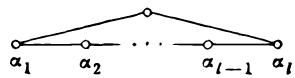
\includegraphics[keepaspectratio]{images/part002_112fabda.jpg}}

当 \(l = 1\) 时，仿射 Weyl 群的 Coxeter 图为

\pandocbounded{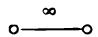
\includegraphics[keepaspectratio]{images/part002_c1e413d9.jpg}}

\begin{enumerate}
\def\labelenumi{(\Alph{enumi})}
\setcounter{enumi}{21}
\tightlist
\item
  \(R^{\prime} = R,\)
\end{enumerate}

\[
\Phi_ {\mathrm{R}} (x, y) = \frac {(x | y)}{2 (l + 1)}, \quad \gamma (\mathrm{R}) = (l + 1) ^ {2}.
\]

\begin{enumerate}
\def\labelenumi{(\Roman{enumi})}
\setcounter{enumi}{5}
\tightlist
\item
  基本权：
\end{enumerate}

\[
\begin{array}{l} \omega_ {i} = \varepsilon_ {1} + \dots + \varepsilon_ {i} - \frac {i}{l + 1} \sum_ {j = 1} ^ {l + 1} \varepsilon_ {j} \\ = \frac {1}{l + 1} [ (l - i + 1) (\alpha_ {1} + 2 \alpha_ {2} + \dots + (i - 1) \alpha_ {i - 1}) \\ \qquad + i ((l - i + 1) \alpha_ {i} + (l - i) \alpha_ {i + 1} + \dots + \alpha_ {l}) ]. \end{array}
\]

\begin{enumerate}
\def\labelenumi{(\Roman{enumi})}
\setcounter{enumi}{6}
\tightlist
\item
  正根之和：
\end{enumerate}

\[
\begin{array}{c} 2 \rho = l \varepsilon_ {1} + (l - 2) \varepsilon_ {2} + (l - 4) \varepsilon_ {3} + \dots - (l - 2) \varepsilon_ {l} - l \varepsilon_ {l + 1} \\ = l \alpha_ {1} + 2 (l - 1) \alpha_ {2} + \dots + i (l - i + 1) \alpha_ {i} + \dots + l \alpha_ {l}. \end{array}
\]

\begin{enumerate}
\def\labelenumi{(\Roman{enumi})}
\setcounter{enumi}{7}
\item
  Q(R)：坐标为整数且和为零的向量集。P(R)：由 Q(R) 与 \(\varepsilon_{1} - (l + 1)^{-1}(\varepsilon_{1} + \varepsilon_{2} + \cdots + \varepsilon_{l+1})\) 生成。P(R)/Q(R) 同构于 Z/(l+1)Z。连接指标：l + 1。
\item
  指数：1, 2, \ldots, l。
\item
  \(\mathrm{W}(\mathrm{R}) = \mathfrak{S}_{l + 1}\) ，可识别为 \(\varepsilon_{i}\) 的置换群。其阶为 \(\mathrm{W}(\mathrm{R})\colon (l + 1)!\)
\item
  \(l = 1\) : A(R) = W(R); \(w_0 = -1\) .
\end{enumerate}

\(l \geqslant 2: A(R) = W(R) \times \{1, -1\} \text{ 且 } w_{0} \text{ 将 } \alpha_{i} \text{ 变为 } -\alpha_{l+1-i}.\)

\begin{enumerate}
\def\labelenumi{(\Roman{enumi})}
\setcounter{enumi}{11}
\item
  群 \(\mathrm{P}(\mathrm{R}^{-})/\mathrm{Q}(\mathrm{R}^{-})\) 是阶为 \((l+1)\) 的循环群；它通过循环置换作用于扩展 Dynkin 图。当 \(l \geqslant 2\) 时，\(\mathrm{A}(\mathrm{R})/\mathrm{W}(\mathrm{R})\) 的唯一非恒等元作用于 \(\mathrm{P}(\mathrm{R})/\mathrm{Q}(\mathrm{R})\)，所用自同构为 \(x \mapsto -x\)。
\item
  Cartan 矩阵 \((l \times l)\) ：
\end{enumerate}

\[
\left( \begin{array}{c c c c c c c} 2 & - 1 & 0 & 0 & \dots & 0 & 0 \\ - 1 & 2 & - 1 & 0 & \dots & 0 & 0 \\ 0 & - 1 & 2 & - 1 & \dots & 0 & 0 \\ 0 & 0 & - 1 & 2 & \dots & 0 & 0 \\ \vdots & \vdots & \vdots & \vdots & \ddots & \vdots & \vdots \\ 0 & 0 & 0 & 0 & \dots & - 1 & 2 \end{array} \right)
\]

\specialchapter{\texorpdfstring{图版 II. \(B_{l}\) 型根系（\(l \geqslant 2\)）}{图版 II. B\_l 型根系 (l >= 2)}}

\begin{enumerate}
\def\labelenumi{(\Roman{enumi})}
\item
  \(V = E = R^{l}\) 。根：\(\pm\varepsilon_{i}, (1\leqslant i\leqslant l), \pm\varepsilon_{i}\pm\varepsilon_{j} (1\leqslant i<j\leqslant l).\) 根的数目：\(n = 2l^{2}\) 。
\item
  基：\(\alpha_{1} = \varepsilon_{1} - \varepsilon_{2},\alpha_{2} = \varepsilon_{2} - \varepsilon_{3},\ldots ,\alpha_{l - 1} = \varepsilon_{l - 1} - \varepsilon_{l},\alpha_{l} = \varepsilon_{l}\) 。正根：
\end{enumerate}

\[
\varepsilon_ {i} = \sum_ {i \leqslant k \leqslant l} \alpha_ {k} (1 \leqslant i \leqslant l),
\]

\[
\varepsilon_ {i} - \varepsilon_ {j} = \sum_ {i \leqslant k <   j} \alpha_ {k} (1 \leqslant i <   j \leqslant l),
\]

\[
\varepsilon_ {i} + \varepsilon_ {j} = \sum_ {i \leqslant k <   j} \alpha_ {k} + 2 \sum_ {j \leqslant k \leqslant l} \alpha_ {k} (1 \leqslant i <   j \leqslant l),
\]

\begin{enumerate}
\def\labelenumi{(\Roman{enumi})}
\setcounter{enumi}{2}
\item
  Coxeter 数：\(h = 2l\) 。
\item
  最高根：
\end{enumerate}

\[
\tilde {\alpha} = \varepsilon_ {1} + \varepsilon_ {2} = \alpha_ {1} + 2 \alpha_ {2} + 2 \alpha_ {3} + \dots + 2 \alpha_ {l}.
\]

有 \(\tilde{\alpha} = 2\omega_{2}\)，当 \(l = 2\) 时；有 \(\tilde{\alpha} = \omega_{2}\)，当 \(l \geqslant 3\) 时。

扩展 Dynkin 图：

当 \(l = 2\) 时：

\pandocbounded{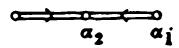
\includegraphics[keepaspectratio]{images/part002_ab2e3717.jpg}}

当 \(l\geqslant 3\) 时

\pandocbounded{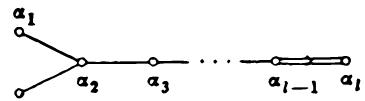
\includegraphics[keepaspectratio]{images/part002_677d35e2.jpg}}

\begin{enumerate}
\def\labelenumi{(\Alph{enumi})}
\setcounter{enumi}{21}
\tightlist
\item
  \(R^{\prime}\) 是向量集
\end{enumerate}

\[
\pm 2 \varepsilon_ {i} (1 \leqslant i \leqslant l), \pm \varepsilon_ {i} \pm \varepsilon_ {j} (1 \leqslant i <   j \leqslant l).
\]

\[
\Phi_ {\mathrm{R}} (x, y) = \frac {(x | y)}{4 l - 2}, \quad \gamma (\mathrm{R}) = (l + 1) (4 l - 2).
\]

\begin{enumerate}
\def\labelenumi{(\Roman{enumi})}
\setcounter{enumi}{5}
\tightlist
\item
  基本权：
\end{enumerate}

\[
\begin{array}{l} \omega_ {i} = \varepsilon_ {1} + \varepsilon_ {2} + \dots + \varepsilon_ {i} (1 \leqslant i <   l) \\ \quad = \alpha_ {1} + 2 \alpha_ {2} + \dots + (i - 1) \alpha_ {i - 1} + i (\alpha_ {i} + \alpha_ {i + 1} + \dots + \alpha_ {l}) \\ \omega_ {l} = \frac {1}{2} (\varepsilon_ {1} + \varepsilon_ {2} + \dots + \varepsilon_ {l}) \\ \quad = \frac {1}{2} (\alpha_ {1} + 2 \alpha_ {2} + \dots + l \alpha_ {l}). \end{array}
\]

\begin{enumerate}
\def\labelenumi{(\Roman{enumi})}
\setcounter{enumi}{6}
\tightlist
\item
  正根之和：
\end{enumerate}

\[
\begin{array}{l} 2 \rho = (2 l - 1) \varepsilon_ {1} + (2 l - 3) \varepsilon_ {2} + \dots + 3 \varepsilon_ {l - 1} + \varepsilon_ {l} \\ = (2 l - 1) \alpha_ {1} + 2 (2 l - 2) \alpha_ {2} + \dots + i (2 l - i) \alpha_ {i} + \dots + l ^ {2} \alpha_ {l}. \end{array}
\]

\begin{enumerate}
\def\labelenumi{(\Roman{enumi})}
\setcounter{enumi}{7}
\tightlist
\item
  \(\mathrm{Q}(\mathrm{R}) = \bigoplus_{i=1}^{l}\mathbf{Z}\varepsilon_i,\mathrm{P}(\mathrm{R}) = \bigoplus_{i=1}^{l}\mathbf{Z}\varepsilon_i + \mathbf{Z}(\frac{1}{2}\sum_{i=1}^{l}\varepsilon_i).\)
\end{enumerate}

\(P(R)/Q(R)\) 同构于 Z/2Z，由 \(\omega_{l}\) 的像生成。连接指标：2。

\begin{enumerate}
\def\labelenumi{(\Roman{enumi})}
\setcounter{enumi}{8}
\item
  指数：1, 3, 5, \ldots, 2l - 1。
\item
  W(R) 是群 \(S_{l}\)（通过对 \(\varepsilon_{i}\) 进行置换作用）与群 \((\mathbf{Z}/2\mathbf{Z})^{l}\)（通过 \(\varepsilon_{i} \mapsto (\pm1)_{i}\varepsilon_{i}\) 作用）的半直积。其阶为 \(2^{l}.l!\)
\item
  A(R) = W(R); \(w_{0} = -1\) .
\item
  \(P(R^{\prime})/Q(R^{\prime})\) 的唯一非平凡元确定扩展 Dynkin 图的唯一非平凡自同构。
\item
  Cartan 矩阵 \((l \times l)\) ：
\end{enumerate}

\[
\left( \begin{array}{c c c c c c c} 2 & - 1 & 0 & 0 & \dots & 0 & 0 \\ - 1 & 2 & - 1 & 0 & \dots & 0 & 0 \\ 0 & - 1 & 2 & - 1 & \dots & 0 & 0 \\ 0 & 0 & - 1 & 2 & \dots & 0 & 0 \\ \vdots & \vdots & \vdots & \vdots & \ddots & \vdots & \vdots \\ 0 & 0 & 0 & 0 & \dots & 2 & - 2 \\ 0 & 0 & 0 & 0 & \dots & - 1 & 2 \end{array} \right)
\]

\specialchapter{\texorpdfstring{图版 III. \(C_l\) 型根系（\(l \geqslant 2\)）}{图版 III. C\_l 型根系 (l >= 2)}}

\begin{enumerate}
\def\labelenumi{(\Roman{enumi})}
\item
  \(V = E = R^{l}.\) 根：\(\pm2\varepsilon_{i}\) 。 （ \(1\leqslant i\leqslant l\) ）。\(\pm\varepsilon_{i}\pm\varepsilon_{j}\)（ \(1\leqslant i<j\leqslant l\) ）。根的数目：\(n = 2l^{2}\) 。
\item
  基：\(\alpha_{1} = \varepsilon_{1} - \varepsilon_{2},\alpha_{2} = \varepsilon_{2} - \varepsilon_{3},\ldots ,\alpha_{l - 1} = \varepsilon_{l - 1} - \varepsilon_{l},\alpha_{l} = 2\varepsilon_{l}\) 。正根：
\end{enumerate}

\[
\varepsilon_ {i} - \varepsilon_ {j} = \sum_ {i \leqslant k <   j} \alpha_ {k} (1 \leqslant i <   j \leqslant l),
\]

\[
\varepsilon_ {i} + \varepsilon_ {j} = \sum_ {i \leqslant k <   j} \alpha_ {k} + 2 \sum_ {j \leqslant k <   l} \alpha_ {k} + \alpha_ {l} (1 \leqslant i <   j \leqslant l),
\]

\[
2 \varepsilon_ {i} = \sum_ {i \leqslant k <   l} \alpha_ {k} + \alpha_ {l} (1 \leqslant i \leqslant l).
\]

\begin{enumerate}
\def\labelenumi{(\Roman{enumi})}
\setcounter{enumi}{2}
\item
  Coxeter 数：\(h = 2l\) 。
\item
  最高根：
\end{enumerate}

\[
\tilde {\alpha} = 2 \varepsilon_ {1} = 2 \alpha_ {1} + 2 \alpha_ {2} + \dots + 2 \alpha_ {l - 1} + \alpha_ {l}.
\]

扩展 Dynkin 图：

\[
\alpha_ {1} \quad \alpha_ {2} \quad \dots \quad \alpha_ {l - 2} \quad \alpha_ {l - 1} \quad \alpha_ {l}
\]

\begin{enumerate}
\def\labelenumi{(\Alph{enumi})}
\setcounter{enumi}{21}
\tightlist
\item
  \(R^{\prime}\) 是向量集 \(\pm\varepsilon_{i}\) 。\(\pm\varepsilon_{i}\pm\varepsilon_{j}\) 。
\end{enumerate}

\[
\Phi_ {\mathrm{R}} (x, y) = \frac {(x | y)}{4 (l + 1)}, \quad \gamma (\mathrm{R}) = (l + 1) (4 l - 2).
\]

\begin{enumerate}
\def\labelenumi{(\Roman{enumi})}
\setcounter{enumi}{5}
\tightlist
\item
  基本权：
\end{enumerate}

\[
\begin{array}{r l} \omega_ {i} & = \varepsilon_ {1} + \varepsilon_ {2} + \dots + \varepsilon_ {i} (1 \leqslant i \leqslant l) \\ & = \alpha_ {1} + 2 \alpha_ {2} + \dots + (i - 1) \alpha_ {i - 1} \\ & \quad + i (\alpha_ {i} + \alpha_ {i + 1} + \dots + \alpha_ {l - 1} + \frac {1}{2} \alpha_ {l}). \end{array}
\]

\begin{enumerate}
\def\labelenumi{(\Roman{enumi})}
\setcounter{enumi}{6}
\tightlist
\item
  正根之和：
\end{enumerate}

\[
\begin{array}{r l} 2 \rho & = 2 l \varepsilon_ {1} + (2 l - 2) \varepsilon_ {2} + \dots + 4 \varepsilon_ {l - 1} + 2 \varepsilon_ {l} \\ & = 2 l \alpha_ {1} + 2 (2 l - 1) \alpha_ {2} + \dots + i (2 l - i + 1) \alpha_ {i} + \dots \\ & \qquad \dots + (l - 1) (l + 2) \alpha_ {l - 1} + \frac {1}{2} l (l + 1) \alpha_ {l}. \end{array}
\]

\begin{enumerate}
\def\labelenumi{(\Roman{enumi})}
\setcounter{enumi}{7}
\item
  Q(R)：坐标为整数且和为偶数的点集。\(P(R) = \bigoplus_{i=1}^{l} Z \varepsilon_i\) 。\(P(R)/Q(R)\) 同构于 \(Z/2Z\)，由 \(\omega_1\) 的像生成。\\
  连接指标：2。
\item
  指数：1, 3, 5, \ldots, 2l - 1。
\item
  W(R) 是群 \(S_{l}\)（通过对 \(\varepsilon_{i}\) 进行置换作用）与群 \((\mathbf{Z}/2\mathbf{Z})^{l}\)（通过 \(\varepsilon_{i} \mapsto (\pm1)_{i}\varepsilon_{i}\) 作用）的半直积。其阶为 \(2^{l}.l!\)
\item
  A(R) = W(R); \(w_{0} = -1\) .
\item
  \(P(R^{-})/Q(R^{-})\) 的唯一非平凡元确定扩展 Dynkin 图的唯一非平凡自同构。
\item
  Cartan 矩阵 \((l\times l)\) ：
\end{enumerate}

\[
\left( \begin{array}{c c c c c c c} 2 & - 1 & 0 & 0 & \dots & 0 & 0 \\ - 1 & 2 & - 1 & 0 & \dots & 0 & 0 \\ 0 & - 1 & 2 & - 1 & \dots & 0 & 0 \\ 0 & 0 & - 1 & 2 & \dots & 0 & 0 \\ \vdots & \vdots & \vdots & \vdots & \ddots & \vdots & \vdots \\ 0 & 0 & 0 & 0 & \dots & 2 & - 1 \\ 0 & 0 & 0 & 0 & \dots & - 2 & 2 \end{array} \right)
\]

\specialchapter{\texorpdfstring{图版 IV. \(D_{l}\) 型根系（\(l \geqslant 3\)）}{图版 IV. D\_l 型根系 (l >= 3)}}

\begin{enumerate}
\def\labelenumi{(\Roman{enumi})}
\tightlist
\item
  \(V = E = R^{l}\) 。根：\(\pm\varepsilon_{i}\pm\varepsilon_{j}(1\leqslant i<j\leqslant l)\)；（ \(\varepsilon_{i}\) ）是 \(R^{l}\) 的标准基。根的数目：\(n = 2l(l - 1)\) 。
\end{enumerate}

\begin{enumerate}
\def\labelenumi{(\Roman{enumi})}
\setcounter{enumi}{1}
\tightlist
\item
  基：\(\alpha_{1} = \varepsilon_{1} - \varepsilon_{2},\alpha_{2} = \varepsilon_{2} - \varepsilon_{3},\ldots ,\alpha_{l - 1} = \varepsilon_{l - 1} - \varepsilon_{l},\alpha_{l} = \varepsilon_{l - 1} + \varepsilon_{l}\) 。正根：
\end{enumerate}

\[
\varepsilon_ {i} - \varepsilon_ {j} = \sum_ {i <   k <   j} \alpha_ {k} (1 \leqslant i <   j \leqslant l).
\]

\[
\varepsilon_ {i} + \varepsilon_ {l} = \sum_ {i \leqslant k \leqslant l - 2} \alpha_ {k} + \alpha_ {l} (1 \leqslant i <   l),
\]

\[
\varepsilon_ {i} + \varepsilon_ {j} = \sum_ {i \leqslant k <   j} \alpha_ {k} + 2 \sum_ {j \leqslant k <   l - 1} \alpha_ {k} + \alpha_ {l - 1} + \alpha_ {l} (1 \leqslant i <   j <   l).
\]

\begin{enumerate}
\def\labelenumi{(\Roman{enumi})}
\setcounter{enumi}{2}
\item
  Coxeter 数：\(h = 2l - 2\) 。
\item
  最高根：
\end{enumerate}

\[
\tilde {\alpha} = \varepsilon_ {1} + \varepsilon_ {2} = \alpha_ {1} + 2 \alpha_ {2} + \dots + 2 \alpha_ {l - 2} + \alpha_ {l - 1} + \alpha_ {l}.
\]

有 \(\tilde{\alpha} = \omega_2 + \omega_3\)，当 \(l = 3\) 时；有 \(\tilde{\alpha} = \omega_2\)，当 \(l \geqslant 4\) 时。

扩展 Dynkin 图（l ≥ 4）：

\pandocbounded{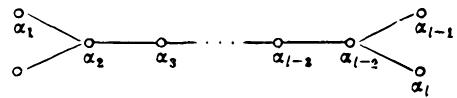
\includegraphics[keepaspectratio]{images/part002_b62b20f1.jpg}}

\begin{enumerate}
\def\labelenumi{(\Alph{enumi})}
\setcounter{enumi}{21}
\tightlist
\item
  \(R^{\prime} = R.\)
\end{enumerate}

\[
\Phi_ {R} (x, y) = \frac {(x | y)}{4 (l - 1)}, \quad \gamma (R) = 4 (l - 1) ^ {2}.
\]

\begin{enumerate}
\def\labelenumi{(\Roman{enumi})}
\setcounter{enumi}{5}
\tightlist
\item
  基本权：
\end{enumerate}

\[
\begin{array}{r l} \omega_ {i} & = \varepsilon_ {1} + \varepsilon_ {2} + \dots + \varepsilon_ {i} (1 \leqslant i \leqslant l - 2) \\ & = \alpha_ {1} + 2 \alpha_ {2} + \dots + (i - 1) \alpha_ {i - 1} + i (\alpha_ {i} + \alpha_ {i + 1} + \dots + \alpha_ {l - 2}) \\ & \quad + \frac {1}{2} i (\alpha_ {l - 1} + \alpha_ {l}) \\ \omega_ {l - 1} & = \frac {1}{2} (\varepsilon_ {1} + \varepsilon_ {2} + \dots + \varepsilon_ {l - 2} + \varepsilon_ {l - 1} - \varepsilon_ {l}) \\ & = \frac {1}{2} (\alpha_ {1} + 2 \alpha_ {2} + \dots + (l - 2) \alpha_ {l - 2} + \frac {1}{2} l \alpha_ {l - 1} + \frac {1}{2} (l - 2) \alpha_ {l}) \\ \omega_ {l} & = \frac {1}{2} (\varepsilon_ {1} + \varepsilon_ {2} + \dots + \varepsilon_ {l - 2} + \varepsilon_ {l - 1} + \varepsilon_ {l}) \\ & = \frac {1}{2} (\alpha_ {1} + 2 \alpha_ {2} + \dots + (l - 2) \alpha_ {l - 2} + \frac {1}{2} (l - 2) \alpha_ {l - 1} + \frac {1}{2} l \alpha_ {l}). \end{array}
\]

\begin{enumerate}
\def\labelenumi{(\Roman{enumi})}
\setcounter{enumi}{6}
\tightlist
\item
  正根之和：
\end{enumerate}

\[
\begin{array}{r l} 2 \rho & = 2 (l - 1) \varepsilon_ {1} + 2 (l - 2) \varepsilon_ {2} + \dots + 2 \varepsilon_ {l - 1} \\ & = 2 (l - 1) \alpha_ {1} + 2 (2 l - 3) \alpha_ {2} + \dots + 2 (i l - \frac {i (i + 1)}{2}) \alpha_ {i} + \dots \\ & \qquad \dots + \frac {l (l - 1)}{2} (\alpha_ {l - 1} + \alpha_ {l}). \end{array}
\]

\begin{enumerate}
\def\labelenumi{(\Roman{enumi})}
\setcounter{enumi}{7}
\tightlist
\item
  Q(R)：坐标为整数且和为偶数的点集。
\end{enumerate}

\[
\mathrm{P} (\mathrm{R}) = \bigoplus_ {i = 1} ^ {l} \mathbf {Z} \varepsilon_ {i} + \mathbf {Z} \left(\frac {1}{2} \sum_ {i = 1} ^ {l} \varepsilon_ {i}\right).
\]

l 为奇数时：\(\mathrm{P}(\mathrm{R})/\mathrm{Q}(\mathrm{R})\) 同构于 Z/4Z，由 \(\omega_{l}\) 的像生成；有 \(\omega_{1} \equiv 2\omega_{l}\) 和 \(\omega_{l-1} \equiv 3\omega_{l} \mod Q(\mathrm{R})\)。l 为偶数时：\(\mathrm{P}(\mathrm{R})/\mathrm{Q}(\mathrm{R})\) 同构于 \((\mathbf{Z}/2\mathbf{Z}) \times (\mathbf{Z}/2\mathbf{Z})\)；阶为 2 的三个元素是 \(\omega_{1}, \omega_{l-1}\) 和 \(\omega_{l}\) 的像。连接指标：4。

\begin{enumerate}
\def\labelenumi{(\Roman{enumi})}
\setcounter{enumi}{8}
\item
  指数：1, 3, 5, \ldots, 2l - 5, 2l - 3, l - 1（最后一个在 l 为偶数时出现两次，在 l 为奇数时出现一次）。
\item
  W(R) 是群 \(S_{l}\)（通过对 \(\varepsilon_{i}\) 进行置换作用）与群 \((\mathbf{Z}/2\mathbf{Z})^{l-1}\)（通过 \(\varepsilon_{i} \mapsto (\pm1)_{i}\varepsilon_{i}\) 作用，并满足 \(\prod_{i}(\pm1)_{i} = 1\)）的半直积。其阶为 \(2^{l-1}.l!\)
\item
  \(l \neq 4\)：A(R)/W(R) = Z/2Z 通过交换节点 \(\alpha_{l-1}\) 和 \(\alpha_l\) 作用于 Dynkin 图。\(l = 4\)：A(R)/W(R) = \(\mathfrak{S}_3\)，通过置换节点 \(\alpha_1, \alpha_3\) 和 \(\alpha_4\) 作用于 Dynkin 图。\(w_0 = -1\) 在 \(l\) 为偶数时成立；\(w_0 = -\varepsilon\) 在 \(l\) 为奇数时成立，其中 \(\varepsilon\) 是交换 \(\alpha_{l-1}\) 与 \(\alpha_l\) 并固定其余 \(\alpha_i\) 的自同构。
\item
  \(\mathrm{P}(\mathbb{R}^{-}) / \mathrm{Q}(\mathbb{R}^{-}) = \mathrm{P}(\mathbb{R}) / \mathrm{Q}(\mathbb{R})\) 在扩展 Dynkin 图上的作用：\(l\) 为奇数时，\(\omega_l\) 将 \(\alpha_0\) 变为 \(\alpha_1\)，将 \(\alpha_l\) 变为 \(\alpha_1\)，将 \(\alpha_1\) 变为 \(\alpha_{l-1}\)，并将 \(\alpha_{l-1}\) 变为 \(\alpha_0\)；它交换 \(\alpha_j\) 和 \(\alpha_{l-j}\)，其中 \(2 \leqslant j \leqslant l - 2\)。\(l\) 为偶数时，\(\omega_l\)（分别为 \(\omega_{l-1}\)）交换 \(\alpha_0\) 和 \(\alpha_l\)（分别为 \(\alpha_0\) 和 \(\alpha_{l-1}\)）、\(\alpha_1\) 和 \(\alpha_{l-1}\)（分别为 \(\alpha_1\) 和 \(\alpha_l\)），并交换 \(\alpha_j\) 和 \(\alpha_{l-j}\)，其中 \(2 \leqslant j \leqslant l - 2\)。
\end{enumerate}

\[
\left( \begin{array}{c c c c c c c} 2 & - 1 & \dots & 0 & 0 & 0 & 0 \\ - 1 & 2 & \dots & 0 & 0 & 0 & 0 \\ \vdots & \vdots & \ddots & \vdots & \vdots & \vdots & \vdots \\ 0 & 0 & \dots & 2 & - 1 & 0 & 0 \\ 0 & 0 & \dots & - 1 & 2 & - 1 & - 1 \\ 0 & 0 & \dots & 0 & - 1 & 2 & 0 \\ 0 & 0 & \dots & 0 & - 1 & 0 & 2 \end{array} \right)
\]

\begin{enumerate}
\def\labelenumi{(\Roman{enumi})}
\setcounter{enumi}{12}
\tightlist
\item
  Cartan 矩阵 \((l\times l)\) ：
\end{enumerate}

\specialchapter{\texorpdfstring{图版 V. \(E_{6}\) 型根系}{图版 V. E\_6 型根系}}

\begin{enumerate}
\def\labelenumi{(\Roman{enumi})}
\tightlist
\item
  V 是 \(E = R^{8}\) 的子空间，由坐标 \((\xi_{i})\) 满足 \(\xi_{6} = \xi_{7} = -\xi_{8}\) 的点组成。根：\(\pm\varepsilon_{i} \pm \varepsilon_{j} (1 \leqslant i < j \leqslant 5)\)，
\end{enumerate}

\[
\pm \frac {1}{2} (\varepsilon_ {8} - \varepsilon_ {7} - \varepsilon_ {6} + \sum_ {i = 1} ^ {5} (- 1) ^ {\nu (i)} \varepsilon_ {i}) \text {with} \sum_ {i = 1} ^ {5} \nu (i) \text {even.}
\]

根的数目：n = 72。

\begin{enumerate}
\def\labelenumi{(\Roman{enumi})}
\setcounter{enumi}{1}
\tightlist
\item
  基：\(\alpha_{1} = \frac{1}{2} (\varepsilon_{1} + \varepsilon_{8}) - \frac{1}{2} (\varepsilon_{2} + \varepsilon_{3} + \varepsilon_{4} + \varepsilon_{5} + \varepsilon_{6} + \varepsilon_{7}),\alpha_{2} = \varepsilon_{1} + \varepsilon_{2},\alpha_{3} =\) \(\varepsilon_2 - \varepsilon_1,\alpha_4 = \varepsilon_3 - \varepsilon_2,\alpha_5 = \varepsilon_4 - \varepsilon_3,\alpha_6 = \varepsilon_5 - \varepsilon_4.\) 正根：\(\pm \varepsilon_i + \varepsilon_j\) \(1\leqslant i <   j\leqslant 5)\)
\end{enumerate}

\[
\frac {1}{2} \left(\varepsilon_ {8} - \varepsilon_ {7} - \varepsilon_ {6} + \sum_ {i = 1} ^ {5} (- 1) ^ {\nu (i)} \varepsilon_ {i}\right) \text {with} \sum_ {i = 1} ^ {5} \nu (i) \text {even}.
\]

至少有一个系数 \(\geqslant 2\) 的正根（我们把根 \(a\alpha_{1} + b\alpha_{2} + c\alpha_{3} + d\alpha_{4} + e\alpha_{5} + f\alpha_{6}\) 记为 \({ }^{a c d e f}_{b})^{13}\)：

\[
\begin{array}{c c c c c c} 0   1   2   1   0 & 1   1   2   1   0 & 0   1   2   1   1 & 1   2   2   1   0 & 1   1   2   1   1 & 0   1   2   2   1 \\ 1 & 1 & 1 & 1 & 1 & 1 \\ 1   2   2   1   1 & 1   1   2   2   1 & 1   2   2   2   1 & 1   2   3   2   1 & 1   2   3   2   1 \\ 1 & 1 & 1 & 1 & 2 \end{array}
\]

\begin{enumerate}
\def\labelenumi{(\Roman{enumi})}
\setcounter{enumi}{2}
\item
  Coxeter 数：\(h = 12\) 。
\item
  最高根：
\end{enumerate}

\[
\begin{array}{r l} \tilde {\alpha} & = \frac {1}{2} (\varepsilon_ {1} + \varepsilon_ {2} + \varepsilon_ {3} + \varepsilon_ {4} + \varepsilon_ {5} - \varepsilon_ {6} - \varepsilon_ {7} + \varepsilon_ {8}) \\ & = \alpha_ {1} + 2 \alpha_ {2} + 2 \alpha_ {3} + 3 \alpha_ {4} + 2 \alpha_ {5} + \alpha_ {6} = \omega_ {2}. \end{array}
\]

扩展 Dynkin 图：

\pandocbounded{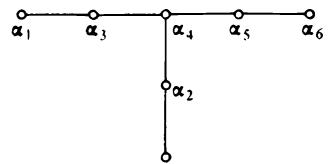
\includegraphics[keepaspectratio]{images/part002_985a73c0.jpg}}

\begin{enumerate}
\def\labelenumi{(\Alph{enumi})}
\setcounter{enumi}{21}
\tightlist
\item
  \(R^{\prime} = R.\)
\end{enumerate}

\[
  \Phi_ {\mathrm{R}} (x, y) = (x | y) / 24, \quad \gamma (\mathrm{R}) = 144.
\]

\begin{enumerate}
\def\labelenumi{(\Roman{enumi})}
\setcounter{enumi}{5}
\tightlist
\item
  基本权：
\end{enumerate}

\[
\begin{array}{l} \omega_ {1} = \frac {2}{3} (\varepsilon_ {8} - \varepsilon_ {7} - \varepsilon_ {6}) = \frac {1}{3} (4 \alpha_ {1} + 3 \alpha_ {2} + 5 \alpha_ {3} + 6 \alpha_ {4} + 4 \alpha_ {5} + 2 \alpha_ {6}) \\ \omega_ {2} = \frac {1}{2} (\varepsilon_ {1} + \varepsilon_ {2} + \varepsilon_ {3} + \varepsilon_ {4} + \varepsilon_ {5} - \varepsilon_ {6} - \varepsilon_ {7} + \varepsilon_ {8}) \\ \quad = \alpha_ {1} + 2 \alpha_ {2} + 2 \alpha_ {3} + 3 \alpha_ {4} + 2 \alpha_ {5} + \alpha_ {6} = \tilde {\alpha} \\ \omega_ {3} = \frac {5}{6} (\varepsilon_ {8} - \varepsilon_ {7} - \varepsilon_ {6}) + \frac {1}{2} (- \varepsilon_ {1} + \varepsilon_ {2} + \varepsilon_ {3} + \varepsilon_ {4} + \varepsilon_ {5}) \\ \quad = \frac {1}{3} (5 \alpha_ {1} + 6 \alpha_ {2} + 10 \alpha_ {3} + 12 \alpha_ {4} + 8 \alpha_ {5} + 4 \alpha_ {6}) \\ \omega_ {4} = \varepsilon_ {3} + \varepsilon_ {4} + \varepsilon_ {5} - \varepsilon_ {6} - \varepsilon_ {7} + \varepsilon_ {8} \\ \quad = 2 \alpha_ {1} + 3 \alpha_ {2} + 4 \alpha_ {3} + 6 \alpha_ {4} + 4 \alpha_ {5} + 2 \alpha_ {6} \\ \omega_ {5} = \frac {2}{3} (\varepsilon_ {8} - \varepsilon_ {7} - \varepsilon_ {6}) + \varepsilon_ {4} + \varepsilon_ {5} \\ \quad = \frac {1}{3} (4 \alpha_ {1} + 6 \alpha_ {2} + 8 \alpha_ {3} + 12 \alpha_ {4} + 10 \alpha_ {5} + 5 \alpha_ {6}) \\ \omega_ {6} = \frac {1}{3} (\varepsilon_ {8} - \varepsilon_ {7} - \varepsilon_ {6}) + \varepsilon_ {5} \\ \quad = \frac {1}{3} (2 \alpha_ {1} + 3 \alpha_ {2} + 4 \alpha_ {3} + 6 \alpha_ {4} + 5 \alpha_ {5} + 4 \alpha_ {6}). \end{array}
\]

\begin{enumerate}
\def\labelenumi{(\Roman{enumi})}
\setcounter{enumi}{6}
\tightlist
\item
  正根之和：
\end{enumerate}

\[
\begin{array}{l} 2 \rho = 2 (\varepsilon_ {2} + 2 \varepsilon_ {3} + 3 \varepsilon_ {4} + 4 \varepsilon_ {5} + 4 (\varepsilon_ {8} - \varepsilon_ {7} - \varepsilon_ {6})) \\ = 2 (8 \alpha_ {1} + 11 \alpha_ {2}) + 15 \alpha_ {3} + 21 \alpha_ {4} + 15 \alpha_ {5} + 8 \alpha_ {6}). \end{array}
\]

\begin{enumerate}
\def\labelenumi{(\Roman{enumi})}
\setcounter{enumi}{7}
\tightlist
\item
  P(R)/Q(R) 同构于 Z/3Z。
\end{enumerate}

连接指标：3。

\begin{enumerate}
\def\labelenumi{(\Roman{enumi})}
\setcounter{enumi}{8}
\item
  指数：1, 4, 5, 7, 8, 11。
\item
  W(R) 的阶：\(2^{7}.3^{4}.5\) 。
\item
  \(\mathrm{A}(\mathrm{R}) = \mathrm{W}(\mathrm{R}) \times \{1, -1\}\)；\(w_0\) 分别将 \(\alpha_1, \alpha_2, \alpha_3, \alpha_4, \alpha_5, \alpha_6\) 变为 \(-\alpha_6, -\alpha_2, -\alpha_5, -\alpha_4, -\alpha_3, -\alpha_1\)。
\item
  \(\mathrm{A}(\mathbb{R}) / \mathrm{W}(\mathbb{R})\) 的非恒等元确定自同构 \(x \mapsto -x\) 在 \(\mathrm{P}(\mathbb{R}) / \mathrm{Q}(\mathbb{R})\) 上的作用。
\end{enumerate}

扩展 Dynkin 图的自同构群同构于 \(S_{3}\)；其阶为 3 的元素由 \(P(R^{-})/Q(R^{-})\) 的两个非平凡元诱导。

\[
\left( \begin{array}{c c c c c c} 2 & 0 & - 1 & 0 & 0 & 0 \\ 0 & 2 & 0 & - 1 & 0 & 0 \\ - 1 & 0 & 2 & - 1 & 0 & 0 \\ 0 & - 1 & - 1 & 2 & - 1 & 0 \\ 0 & 0 & 0 & - 1 & 2 & - 1 \\ 0 & 0 & 0 & 0 & - 1 & 2 \end{array} \right)
\]

\begin{enumerate}
\def\labelenumi{(\Roman{enumi})}
\setcounter{enumi}{12}
\tightlist
\item
  Cartan 矩阵：
\end{enumerate}

\specialchapter{\texorpdfstring{图版 VI. \(E_{7}\) 型根系}{图版 VI. E\_7 型根系}}

\begin{enumerate}
\def\labelenumi{(\Roman{enumi})}
\tightlist
\item
  V 是 \(E = R^{8}\) 中正交于 \(\varepsilon_{7} + \varepsilon_{8}\) 的超平面。
\end{enumerate}

根：\(\pm \varepsilon_{i} \pm \varepsilon_{j} (1 \leqslant i < j \leqslant 6)\)，\(\pm (\varepsilon_{7} - \varepsilon_{8})\)，

\[
\pm \frac {1}{2} (\varepsilon_ {7} - \varepsilon_ {8} + \sum_ {i = 1} ^ {6} (- 1) ^ {\nu (i)} \varepsilon_ {i}) \quad \text { with } \sum_ {i = 1} ^ {8} \nu (i) \text { odd. }
\]

根的数目：n = 126。

\begin{enumerate}
\def\labelenumi{(\Roman{enumi})}
\setcounter{enumi}{1}
\tightlist
\item
  基：
\end{enumerate}

\[
\begin{array}{r l} \alpha_ {1} & = \frac {1}{2} (\varepsilon_ {1} + \varepsilon_ {8}) - \frac {1}{2} (\varepsilon_ {2} + \varepsilon_ {3} + \varepsilon_ {4} + \varepsilon_ {5} + \varepsilon_ {6} + \varepsilon_ {7}), \\ \alpha_ {2} & = \varepsilon_ {1} + \varepsilon_ {2}, \alpha_ {3} = \varepsilon_ {2} - \varepsilon_ {1}, \alpha_ {4} = \varepsilon_ {3} - \varepsilon_ {2}, \alpha_ {5} = \varepsilon_ {4} - \varepsilon_ {3}, \\ \alpha_ {6} & = \varepsilon_ {5} - \varepsilon_ {4}, \alpha_ {7} = \varepsilon_ {6} - \varepsilon_ {5}. \end{array}
\]

正根：

\[
\begin{array}{c} \pm \varepsilon_ {i} + \varepsilon_ {j} (1 \leqslant i <   j \leqslant 6), - \varepsilon_ {7} + \varepsilon_ {8}, \\ \frac {1}{2} (- \varepsilon_ {7} + \varepsilon_ {8} + \sum_ {i = 1} ^ {6} (- 1) ^ {\nu (i)} \varepsilon_ {i}) \quad \text { with } \sum_ {i = 1} ^ {6} \nu (i) \text { odd }. \end{array}
\]

含有 \(\alpha_{7}\) 且至少有一个系数 \(\geqslant 2\) 的正根（我们把根 \(a\alpha_{1} + b\alpha_{2} + c\alpha_{3} + d\alpha_{4} + e\alpha_{5} + f\alpha_{6} + g\alpha_{7}\) 记为 \(\frac{a c d e f g}{b})^{14}\)：

\[
\begin{array}{c c c c c} 0   1   2   1   1   1 & 1   1   2   1   1   1 & 0   1   2   2   1   1 & 1   2   2   1   1   1 & 1   1   2   2   1   1 \\ 1 & 1 & 1 & 1 & 1 \\ 0   1   2   2   2   1 & 1   2   2   2   1   1 & 1   1   2   2   2   1 & 1   2   2   2   2   1 & 1   2   3   2   1   1 \\ 1 & 1 & 1 & 1 & 1 \\ 1   2   3   2   2   1 & 1   2   3   2   1   1 & 1   2   3   3   2   1 & 1   2   3   2   2   1 & 1   2   3   3   2   1 \\ 1 & 2 & 1 & 2 & 2 \end{array}
\]

\[
\begin{array}{c c c} 1 2 4 3 2 1 & 1 3 4 3 2 1 & 2 3 4 3 2 1 \\ 2 & 2 & 2 \end{array}
\]

\begin{enumerate}
\def\labelenumi{(\Roman{enumi})}
\setcounter{enumi}{2}
\item
  Coxeter 数：\(h = 18\) 。
\item
  最高根：
\end{enumerate}

\[
\tilde {\alpha} = \varepsilon_ {8} - \varepsilon_ {7} = 2 \alpha_ {1} + 2 \alpha_ {2} + 3 \alpha_ {3} + 4 \alpha_ {4} + 3 \alpha_ {5} + 2 \alpha_ {6} + \alpha_ {7} = \omega_ {1}.
\]

扩展 Dynkin 图：

\[
\alpha_ {1} \quad \alpha_ {3} \quad \alpha_ {4} \quad \alpha_ {5} \quad \alpha_ {6} \quad \alpha_ {7}
\]

\begin{enumerate}
\def\labelenumi{(\Alph{enumi})}
\setcounter{enumi}{21}
\tightlist
\item
  \(R^{\prime} = R.\)
\end{enumerate}

\[
  \Phi_ {\mathrm{R}} (x, y) = (x | y) / 36, \quad \gamma (\mathrm{R}) = 2 ^ {2}. 3 ^ {4}.
\]

\begin{enumerate}
\def\labelenumi{(\Roman{enumi})}
\setcounter{enumi}{5}
\tightlist
\item
  基本权：
\end{enumerate}

\[
\begin{array}{l} \omega_ {1} = \varepsilon_ {8} - \varepsilon_ {7} = 2 \alpha_ {1} + 2 \alpha_ {2} + 3 \alpha_ {3} + 4 \alpha_ {4} + 3 \alpha_ {5} + 2 \alpha_ {6} + \alpha_ {7} \\ \omega_ {2} = \frac {1}{2} (\varepsilon_ {1} + \varepsilon_ {2} + \varepsilon_ {3} + \varepsilon_ {4} + \varepsilon_ {5} + \varepsilon_ {6} - 2 \varepsilon_ {7} + 2 \varepsilon_ {8}) \\ \qquad = \frac {1}{2} (4 \alpha_ {1} + 7 \alpha_ {2} + 8 \alpha_ {3} + 12 \alpha_ {4} + 9 \alpha_ {5} + 8 \alpha_ {6} + 3 \alpha_ {7}) \\ \omega_ {3} = \frac {1}{2} (- \varepsilon_ {1} + \varepsilon_ {2} + \varepsilon_ {3} + \varepsilon_ {4} + \varepsilon_ {5} + \varepsilon_ {6} - 3 \varepsilon_ {7} + 3 \varepsilon_ {8}) \\ \qquad = 3 \alpha_ {1} + 4 \alpha_ {2} + 6 \alpha_ {3} + 8 \alpha_ {4} + 6 \alpha_ {5} + 4 \alpha_ {6} + 2 \alpha_ {7} \\ \omega_ {4} = \varepsilon_ {3} + \varepsilon_ {4} + \varepsilon_ {5} + \varepsilon_ {6} + 2 (\varepsilon_ {8} - \varepsilon_ {7}) \\ \qquad = 4 \alpha_ {1} + 6 \alpha_ {2} + 8 \alpha_ {3} + 12 \alpha_ {4} + 9 \alpha_ {5} + 6 \alpha_ {6} + 3 \alpha_ {7} \\ \omega_ {5} = \varepsilon_ {4} + \varepsilon_ {5} + \varepsilon_ {6} + \frac {3}{2} (\varepsilon_ {8} - \varepsilon_ {7}) \\ \qquad = \frac {1}{2} (6 \alpha_ {1} + 9 \alpha_ {2} + 12 \alpha_ {3} + 18 \alpha_ {4} + 15 \alpha_ {5} + 10 \alpha_ {6} + 5 \alpha_ {7}) \\ \omega_ {6} = \varepsilon_ {5} + \varepsilon_ {6} - \varepsilon_ {7} + \varepsilon_ {8} \\ \qquad = 2 \alpha_ {1} + 3 \alpha_ {2} + 4 \alpha_ {3} + 6 \alpha_ {4} + 5 \alpha_ {5} + 4 \alpha_ {6} + 2 \alpha_ {7} \\ \omega_ {7} = \varepsilon_ {6} + \frac {1}{2} (\varepsilon_ {8} - \varepsilon_ {7}) \\ \qquad = \frac {1}{2} (2 \alpha_ {1} + 3 \alpha_ {2} + 4 \alpha_ {3} + 6 \alpha_ {4} + 5 \alpha_ {5} + 4 \alpha_ {6} + 3 \alpha_ {7}). \end{array}
\]

\begin{enumerate}
\def\labelenumi{(\Roman{enumi})}
\setcounter{enumi}{6}
\tightlist
\item
  正根之和：
\end{enumerate}

\[
\begin{array}{l} 2 \rho = 2 \varepsilon_ {2} + 4 \varepsilon_ {3} + 6 \varepsilon_ {4} + 8 \varepsilon_ {5} + 10 \varepsilon_ {6} - 17 \varepsilon_ {7} + 17 \varepsilon_ {8} \\ = 34 \alpha_ {1} + 49 \alpha_ {2} + 66 \alpha_ {3} + 96 \alpha_ {4} + 75 \alpha_ {5} + 52 \alpha_ {6} + 27 \alpha_ {7}. \end{array}
\]


\begin{enumerate}
\def\labelenumi{(\Roman{enumi})}
\setcounter{enumi}{7}
\item
  P(R)/Q(R) 同构于 Z/2Z。连接指标：2。
\item
  指数：1, 5, 7, 9, 11, 13, 17。
\item
  W(R) 的阶：\(2^{10}.3^{4}.5.7\) 。
\item
  A(R) = W(R), \(w_{0} = -1\) .
\item
  \(P(R^{\prime})/Q(R^{\prime})\) 只有一个非恒等元：它确定 Dynkin 图的唯一非平凡自同构。
\end{enumerate}

\[
\left( \begin{array}{c c c c c c c} 2 & 0 & - 1 & 0 & 0 & 0 & 0 \\ 0 & 2 & 0 & - 1 & 0 & 0 & 0 \\ - 1 & 0 & 2 & - 1 & 0 & 0 & 0 \\ 0 & - 1 & - 1 & 2 & - 1 & 0 & 0 \\ 0 & 0 & 0 & - 1 & 2 & - 1 & 0 \\ 0 & 0 & 0 & 0 & - 1 & 2 & - 1 \\ 0 & 0 & 0 & 0 & 0 & - 1 & 2 \end{array} \right)
\]

\begin{enumerate}
\def\labelenumi{(\Roman{enumi})}
\setcounter{enumi}{12}
\tightlist
\item
  Cartan 矩阵：
\end{enumerate}

\specialchapter{\texorpdfstring{图版 VII. \(\mathbf{E}_8\) 型根系}{图版 VII. E\_8 型根系}}

\begin{enumerate}
\def\labelenumi{(\Roman{enumi})}
\tightlist
\item
  \(V = E = R^{8}.\)
\end{enumerate}

\[
\begin{array}{l} \text {Roots:} \pm \varepsilon_ {i} \pm \varepsilon_ {j} (i <   j), \frac {1}{2} \sum_ {i = 1} ^ {8} (- 1) ^ {\nu (\mathrm{i})} \varepsilon_ {i} \text {with} \sum_ {i = 1} ^ {8} \nu (i) \text {even.} \\ \text {Number of roots:} n = 240. \end{array}
\]

\begin{enumerate}
\def\labelenumi{(\Roman{enumi})}
\setcounter{enumi}{1}
\tightlist
\item
  基：
\end{enumerate}

\[
\begin{array}{r l} \alpha_ {1} & = \frac {1}{2} (\varepsilon_ {1} + \varepsilon_ {8}) - \frac {1}{2} (\varepsilon_ {2} + \varepsilon_ {3} + \varepsilon_ {4} + \varepsilon_ {5} + \varepsilon_ {6} + \varepsilon_ {7}), \\ \alpha_ {2} & = \varepsilon_ {1} + \varepsilon_ {2}, \alpha_ {3} = \varepsilon_ {2} - \varepsilon_ {1}, \alpha_ {4} = \varepsilon_ {3} - \varepsilon_ {2}, \alpha_ {5} = \varepsilon_ {4} - \varepsilon_ {3}, \\ \alpha_ {6} & = \varepsilon_ {5} - \varepsilon_ {4}, \alpha_ {7} = \varepsilon_ {6} - \varepsilon_ {5}, \alpha_ {8} = \varepsilon_ {7} - \varepsilon_ {6}. \end{array}
\]

正根：

\[
\pm \varepsilon_ {i} + \varepsilon_ {j} (i <   j), \frac {1}{2} (\varepsilon_ {8} + \sum_ {i = 1} ^ {7} (- 1) ^ {\nu (\mathrm{i})} \varepsilon_ {i}) \text {with} \sum_ {i = 1} ^ {7} \nu (i) \text {even}.
\]

含有 \(\alpha_{8}\) 且至少有一个系数 \(\geqslant 2\) 的正根（我们把根 \(a\alpha_{1} + b\alpha_{2} + c\alpha_{3} + d\alpha_{4} + e\alpha_{5} + f\alpha_{6} + g\alpha_{7} + h\alpha_{8}\) 记为 \(\left.\frac{a}{b}c\frac{d}{e}\frac{e}{f}\frac{g}{h}\right)^{15}\)：

\[
\begin{array}{c c c c c} 0   1   2   1   1   1   1 & 0   1   2   2   1   1   1 & 1   1   2   1   1   1   1 & 0   1   2   2   2   1   1 & 1   2   2   1   1   1   1 \\ 1 & 1 & 1 & 1 & 1 \\ 1   1   2   2   1   1   1 & 1   2   2   2   1   1   1 & 1   1   2   2   2   1   1 & 0   1   2   2   2   2   1 & 1   2   3   2   1   1   1 \\ 1 & 1 & 1 & 1 & 1 \\ 1   2   2   2   2   1   1 & 1   1   2   2   2   2   1 & 1   2   3   2   2   1   1 & 1   2   3   2   2   1   1 & 1   2   2   2   2   2   1 \\ 1 & 1 & 2 & 1 & 1 \\ 1   2   3   2   2   1   1 & 1   2   3   3   2   1   1 & 1   2   3   2   2   2   1 & 1   2   3   3   2   1   1 & 1   2   3   2   2   2   1 \\ 2 & 1 & 1 & 2 & 2 \end{array}
\]

\[
\begin{array}{c c c c c} 1   2   3   3   3   2   1 & 1   2   4   3   2   1   1 & 1   2   3   3   2   2   1 & 1   2   3   3   3   2   1 & 1   3   4   3   2   1   1 \\ 1 & 2 & 2 & 1 & 2 \\ 1   2   4   3   2   2   1 & 1   2   3   3   3   2   1 & 2   3   4   3   2   1   1 & 1   3   4   3   2   2   1 & 1   2   4   3   3   2   1 \\ 2 & 2 & 2 & 2 & 2 \\ 2   3   4   3   2   2   1 & 1   3   4   3   3   2   1 & 1   2   4   4   3   2   1 & 2   3   4   3   3   2   1 & 1   3   4   4   3   2   1 \\ 2 & 2 & 2 & 2 & 2 \\ 1   3   5   4   3   2   1 & 2   3   4   4   3   2   1 & 1   3   5   4   3   2   1 & 2   3   5   4   3   2   1 & 2   3   5   4   3   2   1 \\ 2 & 2 & 3 & 2 & 3 \\ \text { } _ {2} ^ {2} \text { } _ {5} ^ {4} \text { } _ {5} ^ {4} \text { } _ {5} ^ {4} \text { } _ {5} ^ {4} \text { } _ {5} ^ {4} \text { } _ {5} ^ {4} \text { } _ {5} ^ {4} \text { } _ {5} ^ {4} \text { } _ {5} ^ {4} \text {(} _ {2} ^ {2} \text {)} _ {2} ^ {3} \text {)} _ {3} ^ {3} \text {)} _ {3} ^ {3} \text {)} _ {3} ^ {3} \end{array}
\]

\begin{enumerate}
\def\labelenumi{(\Roman{enumi})}
\setcounter{enumi}{2}
\item
  Coxeter 数：\(h = 30\) 。
\item
  最高根：
\end{enumerate}

\[
\begin{array}{r l} \tilde {\alpha} & = \varepsilon_ {7} + \varepsilon_ {8} = 2 \alpha_ {1} + 3 \alpha_ {2} + 4 \alpha_ {3} + 6 \alpha_ {4} + 5 \alpha_ {5} + 4 \alpha_ {6} + 3 \alpha_ {7} + 2 \alpha_ {8} \\ & = \omega_ {8}. \end{array}
\]

扩展 Dynkin 图为：

\[
\begin{array}{c} \alpha_ {1} \quad \alpha_ {3} \\ \alpha_ {4} \quad \alpha_ {5} \quad \alpha_ {6} \quad \alpha_ {7} \quad \alpha_ {8} \\ \alpha_ {2} \end{array}
\]

\begin{enumerate}
\def\labelenumi{(\Alph{enumi})}
\setcounter{enumi}{21}
\tightlist
\item
  \(R^{\prime} = R.\)
\end{enumerate}

\[
  \Phi_ {\mathrm{R}} (x, y) = (x | y) / 60, \quad \gamma (\mathrm{R}) = 900.
\]

\begin{enumerate}
\def\labelenumi{(\Roman{enumi})}
\setcounter{enumi}{5}
\tightlist
\item
  基本权：
\end{enumerate}

\[
\begin{array}{l} \omega_ {1} = 2 \varepsilon_ {8} = 4 \alpha_ {1} + 5 \alpha_ {2} + 7 \alpha_ {3} + 10 \alpha_ {4} + 8 \alpha_ {5} + 6 \alpha_ {6} + 4 \alpha_ {7} + 2 \alpha_ {8} \\ \omega_ {2} = \frac {1}{2} (\varepsilon_ {1} + \varepsilon_ {2} + \varepsilon_ {3} + \varepsilon_ {4} + \varepsilon_ {5} + \varepsilon_ {6} + \varepsilon_ {7} + 5 \varepsilon_ {8}) \\ \quad = 5 \alpha_ {1} + 8 \alpha_ {2} + 10 \alpha_ {3} + 15 \alpha_ {4} + 12 \alpha_ {5} + 9 \alpha_ {6} + 6 \alpha_ {7} + 3 \alpha_ {8} \\ \omega_ {3} = \frac {1}{2} (- \varepsilon_ {1} + \varepsilon_ {2} + \varepsilon_ {3} + \varepsilon_ {4} + \varepsilon_ {5} + \varepsilon_ {6} + \varepsilon_ {7} + 7 \varepsilon_ {8}) \\ \quad = 7 \alpha_ {1} + 10 \alpha_ {2} + 14 \alpha_ {3} + 20 \alpha_ {4} + 16 \alpha_ {5} + 12 \alpha_ {6} + 8 \alpha_ {7} + 4 \alpha_ {8} \\ \omega_ {4} = \varepsilon_ {3} + \varepsilon_ {4} + \varepsilon_ {5} + \varepsilon_ {6} + \varepsilon_ {7} + 5 \varepsilon_ {8} \\ \quad = 10 \alpha_ {1} + 15 \alpha_ {2} + 20 \alpha_ {3} + 30 \alpha_ {4} + 24 \alpha_ {5} + 18 \alpha_ {6} + 12 \alpha_ {7} + 6 \alpha_ {8} \end{array}
\]

\[
\begin{array}{r l} \omega_ {5} & = \varepsilon_ {4} + \varepsilon_ {5} + \varepsilon_ {6} + \varepsilon_ {7} + 4 \varepsilon_ {8} \\ & = 8 \alpha_ {1} + 12 \alpha_ {2} + 16 \alpha_ {3} + 24 \alpha_ {4} + 20 \alpha_ {5} + 15 \alpha_ {6} + 10 \alpha_ {7} + 5 \alpha_ {8} \\ \omega_ {6} & = \varepsilon_ {5} + \varepsilon_ {6} + \varepsilon_ {7} + 3 \varepsilon_ {8} \\ & = 6 \alpha_ {1} + 9 \alpha_ {2} + 12 \alpha_ {3} + 18 \alpha_ {4} + 15 \alpha_ {5} + 12 \alpha_ {6} + 8 \alpha_ {7} + 4 \alpha_ {8} \\ \omega_ {7} & = \varepsilon_ {6} + \varepsilon_ {7} + 2 \varepsilon_ {8} \\ & = 4 \alpha_ {1} + 6 \alpha_ {2} + 8 \alpha_ {3} + 12 \alpha_ {4} + 10 \alpha_ {5} + 8 \alpha_ {6} + 6 \alpha_ {7} + 3 \alpha_ {8} \\ \omega_ {8} & = \varepsilon_ {7} + \varepsilon_ {8} \\ & = 5 \alpha_ {1} + 8 \alpha_ {2} + 10 \alpha_ {3} + 15 \alpha_ {4} + 12 \alpha_ {5} + 9 \alpha_ {6} + 6 \alpha_ {7} + 3 \alpha_ {8} = \tilde {\alpha}. \end{array}
\]

\begin{enumerate}
\def\labelenumi{(\Roman{enumi})}
\setcounter{enumi}{6}
\tightlist
\item
  正根之和：
\end{enumerate}

\[
\begin{array}{r l} 2 \rho & = 2 (\varepsilon_ {2} + 2 \varepsilon_ {3} + 3 \varepsilon_ {4} + 4 \varepsilon_ {5} + 5 \varepsilon_ {6} + 6 \varepsilon_ {7} + 23 \varepsilon_ {8}) \\ & = 2 (46 \alpha_ {1} + 68 \alpha_ {2} + 91 \alpha_ {3} + 135 \alpha_ {4} + 110 \alpha_ {5} + 84 \alpha_ {6} + 57 \alpha_ {7} + 29 \alpha_ {8}). \end{array}
\]

\begin{enumerate}
\def\labelenumi{(\Roman{enumi})}
\setcounter{enumi}{7}
\tightlist
\item
  Q(R)：坐标为 \(\xi_{i}\) 且满足 \(2\xi_{i} \in \mathbf{Z}\) 的点集，
\end{enumerate}

\[
\begin{array}{l} \xi_ {i} - \xi_ {j} \in \mathbf {Z}, \sum_ {i = 1} ^ {8} \xi_ {i} \in 2 \mathbf {Z}. \\ \text { Connection   index: } 1. \end{array}
\]

\begin{enumerate}
\def\labelenumi{(\Roman{enumi})}
\setcounter{enumi}{8}
\item
  指数：1, 7, 11, 13, 17, 19, 23, 29。
\item
  W(R) 的阶：\(2^{14}.3^{5}.5^{2}.7\) 。
\item
  以及（XII）\(A(R) = W(R). w_0 = -1.\)
\item
  Cartan 矩阵：
\end{enumerate}

\[
\left( \begin{array}{c c c c c c c c} 2 & 0 & - 1 & 0 & 0 & 0 & 0 & 0 \\ 0 & 2 & 0 & - 1 & 0 & 0 & 0 & 0 \\ - 1 & 0 & 2 & - 1 & 0 & 0 & 0 & 0 \\ 0 & - 1 & - 1 & 2 & - 1 & 0 & 0 & 0 \\ 0 & 0 & 0 & - 1 & 2 & - 1 & 0 & 0 \\ 0 & 0 & 0 & 0 & - 1 & 2 & - 1 & 0 \\ 0 & 0 & 0 & 0 & 0 & - 1 & 2 & - 1 \\ 0 & 0 & 0 & 0 & 0 & 0 & - 1 & 2 \end{array} \right)
\]

\specialchapter{\texorpdfstring{图版 VIII. \(F_{4}\) 型根系}{图版 VIII. F\_4 型根系}}

\begin{enumerate}
\def\labelenumi{(\Roman{enumi})}
\tightlist
\item
  \(V = E = R^4.\)
\end{enumerate}

根：

\[
\begin{array}{c} \pm \varepsilon_ {i}. (1 \leqslant i \leqslant 4), \quad \pm \varepsilon_ {i} \pm \varepsilon_ {j} (1 \leqslant i <   j \leqslant 4), \\ \frac {1}{2} (\pm \varepsilon_ {1} \pm \varepsilon_ {2} \pm \varepsilon_ {3} \pm \varepsilon_ {4}). \end{array}
\]

根的数目：n = 48。

\begin{enumerate}
\def\labelenumi{(\Roman{enumi})}
\setcounter{enumi}{1}
\tightlist
\item
  基：
\end{enumerate}

\[
\alpha_ {1} = \varepsilon_ {2} - \varepsilon_ {3}, \alpha_ {2} = \varepsilon_ {3} - \varepsilon_ {4}, \alpha_ {3} = \varepsilon_ {4}, \alpha_ {4} = \frac {1}{2} (\varepsilon_ {1} - \varepsilon_ {2} - \varepsilon_ {3} - \varepsilon_ {4}).
\]

正根：

\[
\varepsilon_ {i} (1 \leqslant i \leqslant 4), \quad \varepsilon_ {i} \pm \varepsilon_ {j} (1 \leqslant i <   j \leqslant 4). \quad \frac {1}{2} (\varepsilon_ {1} \pm \varepsilon_ {2} \pm \varepsilon_ {3} \pm \varepsilon_ {4}).
\]

至少有一个系数 \(\geqslant2\) 的正根（我们把根 \(a\alpha_{1}+b\alpha_{2}+c\alpha_{3}+d\alpha_{4}\) 记为 abcd）\(^{16}\)：

\[
\begin{array}{c c c c c c c c} 0 1 2 0 & 1 1 2 0 & 0 1 2 1 & 1 2 2 0 & 1 1 2 1 & 0 1 2 2 & 1 2 2 1 & 1 1 2 2 \\ & 1 2 3 1 & 1 2 2 2 & 1 2 3 2 & 1 2 4 2 & 1 3 4 2 & 2 3 4 2 \end{array}
\]

\begin{enumerate}
\def\labelenumi{(\Roman{enumi})}
\setcounter{enumi}{2}
\item
  根的数目：\(h = 12\) 。
\item
  最高根：\(\tilde{\alpha} = \varepsilon_1 + \varepsilon_2 = 2\alpha_1 + 3\alpha_2 + 4\alpha_3 + 2\alpha_4 = \omega_1\) 。扩展 Dynkin 图：
\end{enumerate}

\pandocbounded{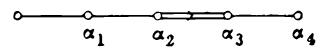
\includegraphics[keepaspectratio]{images/part002_560ef793.jpg}}

\begin{enumerate}
\def\labelenumi{(\Alph{enumi})}
\setcounter{enumi}{21}
\tightlist
\item
  \(R^{\prime}\) 是向量集 \(\pm2\varepsilon_{i},\pm\varepsilon_{i}\pm\varepsilon_{j},\pm\varepsilon_{1}\pm\varepsilon_{2}\pm\varepsilon_{3}\pm\varepsilon_{4}.\)
\end{enumerate}

\[
  \Phi_ {\mathrm{R}} (x, y) = \frac {(x | y)}{18}, \quad \gamma (\mathrm{R}) = 2. 3 ^ {4}.
\]

\begin{enumerate}
\def\labelenumi{(\Roman{enumi})}
\setcounter{enumi}{5}
\tightlist
\item
  基本权：
\end{enumerate}

\[
\omega_ {1} = \varepsilon_ {1} + \varepsilon_ {2} = 2 \alpha_ {1} + 3 \alpha_ {2} + 4 \alpha_ {3} + 2 \alpha_ {4}
\]

\[
\omega_ {2} = 2 \varepsilon_ {1} + \varepsilon_ {2} + \varepsilon_ {3} = 3 \alpha_ {1} + 6 \alpha_ {2} + 8 \alpha_ {3} + 4 \alpha_ {4}
\]

\[
\omega_ {3} = \frac {1}{2} (3 \varepsilon_ {1} + \varepsilon_ {2} + \varepsilon_ {3} + \varepsilon_ {4}) = 2 \alpha_ {1} + 4 \alpha_ {2} + 6 \alpha_ {3} + 3 \alpha_ {4}
\]

\[
\omega_ {4} = \varepsilon_ {1} = \alpha_ {1} + 2 \alpha_ {2} + 3 \alpha_ {3} + 2 \alpha_ {4}.
\]

\begin{enumerate}
\def\labelenumi{(\Roman{enumi})}
\setcounter{enumi}{6}
\tightlist
\item
  正根之和：
\end{enumerate}

\[
2 \rho = 11 \varepsilon_ {1} + 5 \varepsilon_ {2} + 3 \varepsilon_ {3} + \varepsilon_ {4} = 16 \alpha_ {1} + 30 \alpha_ {2} + 42 \alpha_ {3} + 22 \alpha_ {4}.
\]

\begin{enumerate}
\def\labelenumi{(\Roman{enumi})}
\setcounter{enumi}{7}
\tightlist
\item
  \(\mathrm{Q}(\mathrm{R}) = \bigoplus_{i=1}^{4} \mathbf{Z} \varepsilon_i + \mathbf{Z}\left(\frac{1}{2} \sum_{i=1}^{4} \varepsilon_i\right)\) .
\end{enumerate}

\(P(R) = Q(R).\)

连接指标：1。

\begin{enumerate}
\def\labelenumi{(\Roman{enumi})}
\setcounter{enumi}{8}
\item
  指数：1, 5, 7, 11。
\item
  以及（XI）A(R) = W(R)，\(w_{0} = -1\) 。
\item
  Cartan 矩阵：
\end{enumerate}

\[
\left( \begin{array}{c c c c} 2 & - 1 & 0 & 0 \\ - 1 & 2 & - 2 & 0 \\ 0 & - 1 & 2 & - 1 \\ 0 & 0 & - 1 & 2 \end{array} \right)
\]

\specialchapter{\texorpdfstring{图版 IX. \(\mathbf{G}_2\) 型根系}{图版 IX. G\_2 型根系}}

\begin{enumerate}
\def\labelenumi{(\Roman{enumi})}
\tightlist
\item
  V 是 \(E = R^{3}\) 中方程为 \(\xi_{1} + \xi_{2} + \xi_{3} = 0\) 的超平面。根：
\end{enumerate}

\[
\begin{array}{c} \pm (\varepsilon_ {1} - \varepsilon_ {2}), \quad \pm (\varepsilon_ {1} - \varepsilon_ {3}), \quad \pm (\varepsilon_ {2} - \varepsilon_ {3}), \quad \pm (2 \varepsilon_ {1} - \varepsilon_ {2} - \varepsilon_ {3}), \\ \pm (2 \varepsilon_ {2} - \varepsilon_ {1} - \varepsilon_ {3}), \quad \pm (2 \varepsilon_ {3} - \varepsilon_ {1} - \varepsilon_ {2}). \end{array}
\]

根的数目：n = 12。

\begin{enumerate}
\def\labelenumi{(\Roman{enumi})}
\setcounter{enumi}{1}
\item
  基：\(\alpha_{1} = \varepsilon_{1} - \varepsilon_{2},\alpha_{2} = -2\varepsilon_{1} + \varepsilon_{2} + \varepsilon_{3}\) 。正根：\(\alpha_{1},\alpha_{1} + \alpha_{2},2\alpha_{1} + \alpha_{2},3\alpha_{1} + \alpha_{2},3\alpha_{1} + 2\alpha_{2}\) 。
\item
  Coxeter 数：h = 6。
\item
  最高根：\(\tilde{\alpha} = -\varepsilon_1 - \varepsilon_2 + 2\varepsilon_3 = 3\alpha_1 + 2\alpha_2 = \omega_2\) 。扩展 Dynkin 图：
\end{enumerate}

\pandocbounded{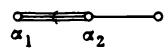
\includegraphics[keepaspectratio]{images/part002_d2921928.jpg}}

\begin{enumerate}
\def\labelenumi{(\Alph{enumi})}
\setcounter{enumi}{21}
\tightlist
\item
  \(R^{\prime}\) 是向量集
\end{enumerate}

\[
\pm \alpha_ {1}, \quad \pm (\alpha_ {1} + \alpha_ {2}), \quad \pm (2 \alpha_ {1} + \alpha_ {2}), \quad \pm \frac {1}{3} \alpha_ {2},
\]

\[
\pm \frac {1}{3} (3 \alpha_ {1} + \alpha_ {2}), \quad \pm \frac {1}{3} (3 \alpha_ {1} + 2 \alpha_ {2}).
\]

\[
  \Phi_ {\mathrm{R}} (x, y) = \frac {(x | y)}{24}, \quad \gamma (\mathrm{R}) = 48.
\]

\begin{enumerate}
\def\labelenumi{(\Roman{enumi})}
\setcounter{enumi}{5}
\tightlist
\item
  基本权：
\end{enumerate}

\[
\omega_ {1} = 2 \alpha_ {1} + \alpha_ {2}, \quad \omega_ {2} = 3 \alpha_ {1} + 2 \alpha_ {2} = \tilde {\alpha}.
\]

\begin{enumerate}
\def\labelenumi{(\Roman{enumi})}
\setcounter{enumi}{6}
\tightlist
\item
  正根之和：
\end{enumerate}

\[
2 \rho = 2 (5 \alpha_ {1} + 3 \alpha_ {2}).
\]

\begin{enumerate}
\def\labelenumi{(\Roman{enumi})}
\setcounter{enumi}{7}
\item
  \(\mathrm{P}(\mathrm{R}) = \mathrm{Q}(\mathrm{R})\) 。连接指标：1。
\item
  指数：1, 5。
\item
  W(R)：阶为 12 的二面体群。
\item
  以及（XII）：A(R) = W(R)。\(w_{0} = -1\) 。
\item
  Cartan 矩阵：
\end{enumerate}

\[
\left( \begin{array}{c c} 2 & - 1 \\ - 3 & 2 \end{array} \right)
\]

\specialchapter{图版 X. 秩为 2 的不可约根系}

\pandocbounded{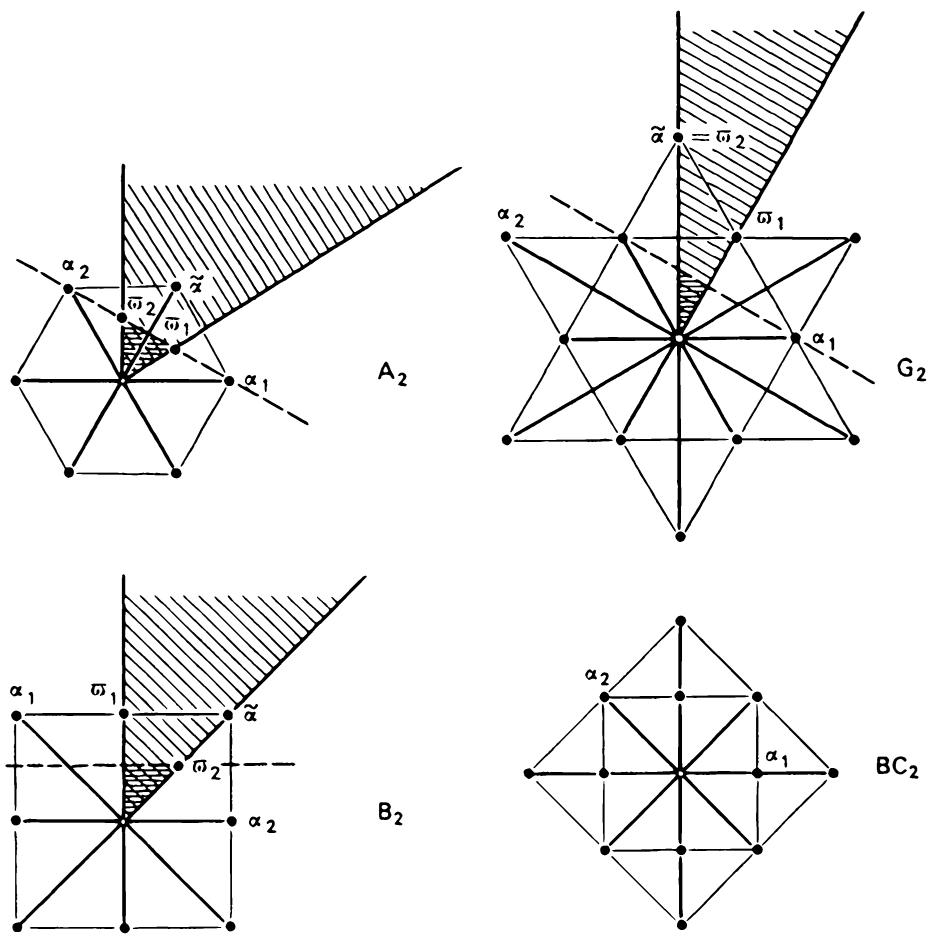
\includegraphics[keepaspectratio]{images/part002_e5dc67b9.jpg}}\\
上面的前三幅图表示 \(A_{2}\)、\(B_{2}\) 和 \(G_{2}\) 类型的根系 R。阴影区域表示与基 \((\alpha_{1},\alpha_{2})\) 相应的室 C。直线 \((x|\beta)=1\)，其中 \(\beta\) 表示

逆根系 \(R^{-}\) 的最高根；该直线以点线表示，双重阴影区域表示包含于 C 且顶点为 0 的 \(R^{-}\) 小室。

最后一幅图表示秩为 2 的唯一不可约非约化根系。
